\newthought{In the first two years} of your mathematical education, you have become familiar with calculus for functions and vector fields on $\R^n$.
As I mentioned in the introduction, euclidean spaces will be our prototypical example.
However, the generalization of calculus to curved spaces will require us to carefully isolate the mathematical structures associated to the various concepts.
This process will help us to discover the rich geometric structure that lies at the root of derivation and integration, which ultimately is of great mathematical interest and has revolutionized mathematical physics.

If you think carefully, this abstraction step was already in the air. Think about the concept of continuity.

\begin{enumerate}[a)]
  \item (High school) A function $f:\R\to\R$ is \emph{continuous} if you can draw it without lifting your pen from the page.
  Then, the derivative $f'(x)$ of $f$ at a point $x$ is just the slope of the function $f$ at the point $x$.
  
  \item (Analysis) A function is continuous if its left and right limits at each point exist and have the same value.
  Then, $f:\R\to\R$ is \emph{differentiable} at a point $x$ if the limit
  \begin{equation}
    f'(x) := \lim_{h\to0} \frac{f(x+h) - f(x)}{h} 
  \end{equation}
  exists, and is \emph{continuously differentiable} if $x\mapsto f'(x)$ is itself a continuous function.
  
  \item (Multivariable analysis) You generalized the concepts to functions with more than one variable.
  Continuity is practically unchanged but, now, a continuous function $f=(f^1, \ldots, f^m):\R^n\to\R^m$ is differentiable at $x=(x^1,\ldots,x^m)\in\R^n$ if there is a \emph{linear map}\footnote{That is, $T$ is a $m\times n$ matrix.} $T: \R^n\to\R^m$ such that
  \begin{equation}\label{eq:diff}
    \lim_{\|h\|\to 0} \frac{\|f(x+h) - f(x) - T h\|}{\|h\|} = 0.
  \end{equation}
  The map $Df(x) := T$ is the \emph{differential} (or total derivative) of $f$ and is nothing else than the Jacobian matrix of $f$ at the point $x$, that is
  \begin{equation}\label{eq:jacobian}
    Df(x) = \begin{pmatrix}
      \frac{\partial f^1}{\partial x^1}(x) & \cdots & \frac{\partial f^1}{\partial x^n}(x) \\
      \vdots & \ddots & \vdots \\
      \frac{\partial f^m}{\partial x^1}(x) & \cdots & \frac{\partial f^m}{\partial x^n}(x) \\
    \end{pmatrix}.
  \end{equation} 
  The notion of continuous differentiability is unchanged\footnote{Note how the spaces are changing though: since it takes values in the space of $m\times n$ matrices, the differential $x\mapsto Df(x)$ is in fact a mapping of $\R^n \to \R^{mn}$.}, and in fact for $m=n=1$ it coincides with the one you gave for real functions.
  
  \item (Metric and topological spaces) A map $f:X\to Y$ between \emph{topological spaces} is continuous if preimages of open sets under $f$ are open. More explicitly, $f$ is continuous if for every open set $O\subset Y$, $f^{-1}(O)\subset X$ is an open set.

  If $X$ and $Y$ are \emph{metric spaces}, then this reduces to the definition given above.
  But how can we make sense of differentiability in this case? 
  
  If you have taken a course on calculus of variations, you know that you can make sense of \eqref{eq:diff} and give a notion of differentiability in the case $X$ and $Y$ are Banach spaces\footnote{Complete normed vector spaces.}.
  In general, a topological space is \emph{not} a vector space: there is no notion of adding points, least of all one of linearity.
\end{enumerate}

This is where differential geometry comes into play.
The rest of this chapter will be devoted to the introduction of \emph{smooth manifolds}, which are a class of topological spaces on which it is possible to make sense of the notion of differentiation even though they are not necessarily vector spaces.
We will do this in two stages.
First we will introduce \emph{topological manifolds}, which are topological spaces that \emph{locally} look like euclidean spaces.
Then we will endow topological manifolds with a so-called \emph{smooth structure}.
This will allow us to define differentiability and \emph{smooth manifolds}\footnote{These will just be topological manifolds with a smooth structure.}.

Without further ado, let's get started.

\section{Topological manifolds}

\newthought{Since to speak of continuity we need topological spaces}, it may be a good idea to remind you what they are and set some notation.
I will be very brief: if you need a more extensive reminder, you can refer to Appendix A of either \cite{book:tu} or \cite{book:lee}.

\begin{definition}
  Let $M$ be some set and $\cT$ a set of subsets of $M$.
  A pair $(M, \cT)$ is a \emph{topological space}\footnote{In such case the elements $O\in\cT$ of $\cT$ are all subsets of $M$ called \emph{open} subsets and $\cT$ is a topology on $X$.} if
  \begin{enumerate}[(i)]
    \item $M$ and $\emptyset$ are open, i.e., $M\in \cT$ and $\emptyset\in\cT$;
    \item arbitrary unions of families of open subsets are open;
    \item the intersection of finitely many\footnote{It is equivalent to require the intersection of any two open subsets to be open. (Why?)} open subsets is open.
  \end{enumerate}
\end{definition}

With topological spaces at hand, we can give a definition of continuity and introduce a way to compare topological spaces.

\begin{definition}
  A map $f: X \to Y$ between two topological spaces $(X,\cT)$ and $(Y, \cU)$ is called:
  \begin{itemize}
    \item \emph{continuous} if $U\in\cU$ implies that $f^{-1}(U)\in\cT$, that is, preimages of open sets under $f$ are open;
    \item \emph{homeomorphism} if it is bijective\footnote{I.e., one-to-one.} and continuous with continuous inverse.\marginnote{The existence of an homeomorphism between two spaces can be thought as those spaces being equivalent in a loose sense: they can be deformed continuously into each other.}
  \end{itemize}
\end{definition}

\begin{marginfigure}
  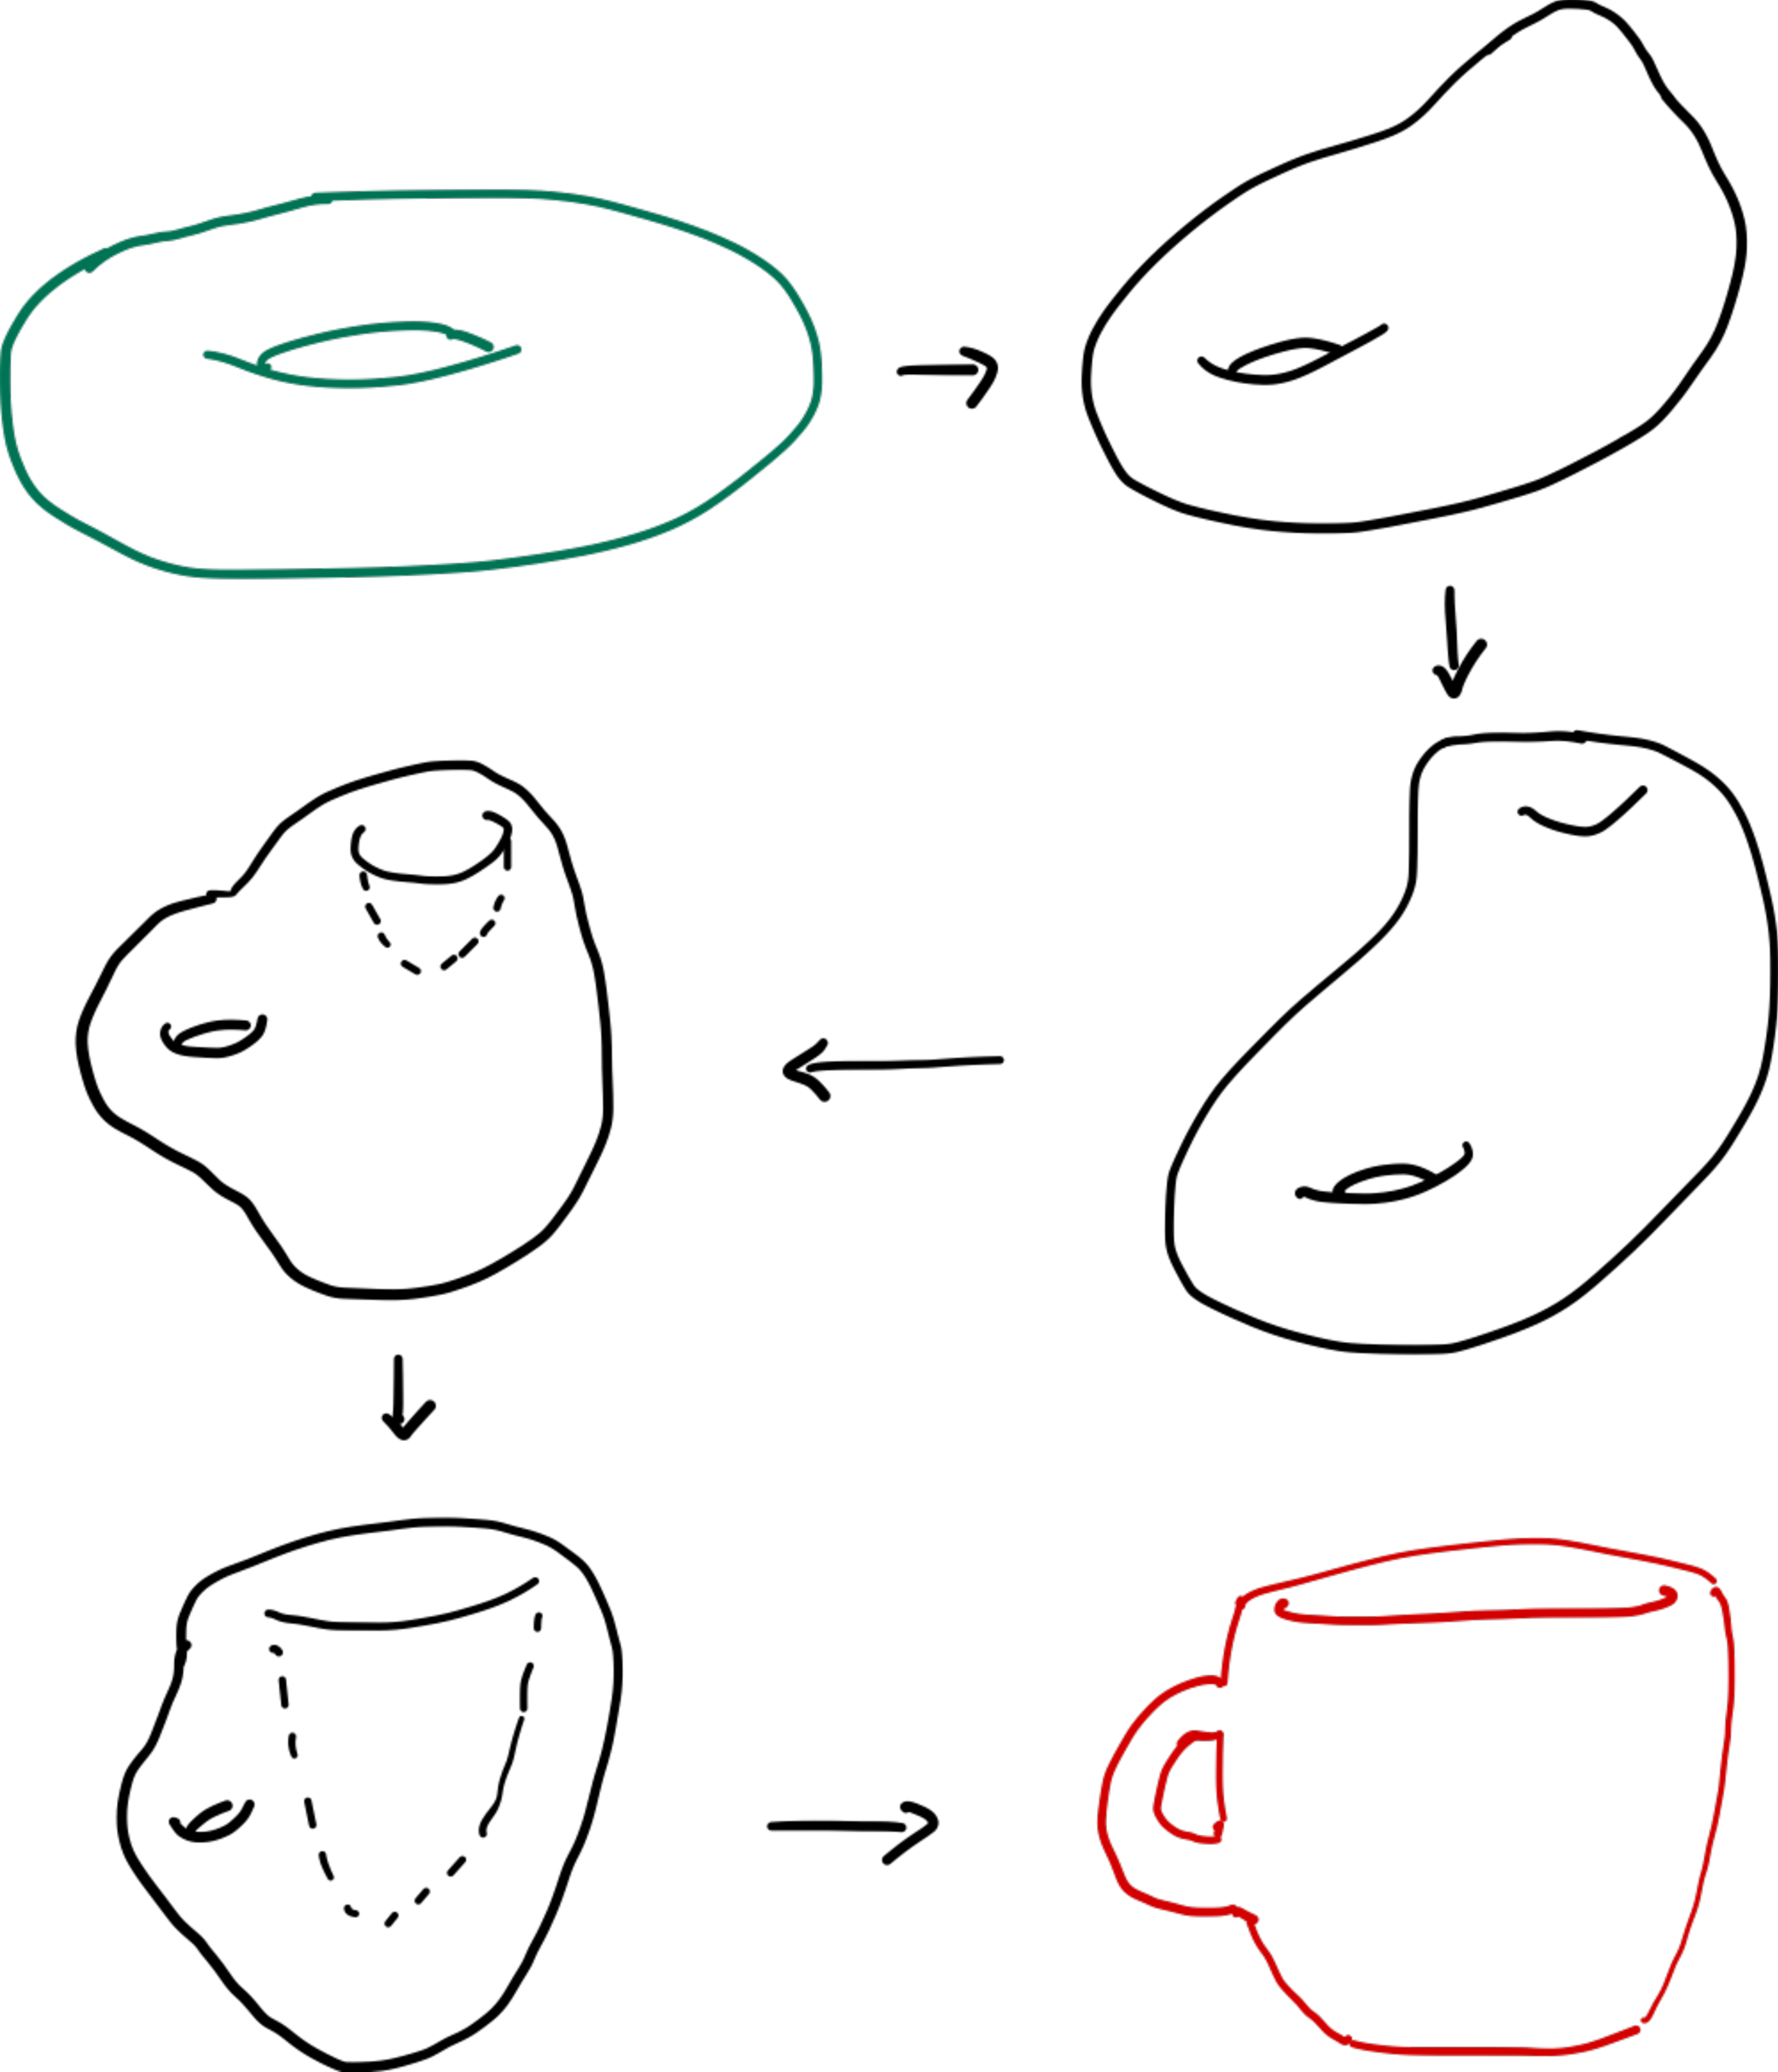
\includegraphics{images/1_1-dount-to-cup.pdf}
  \vspace{5pt}
\end{marginfigure}

\begin{definition}
  A topological space $(X, \cT)$ is \emph{Hausdorff} if every two distinct points admit disjoint open neighbourhoods. That is, for every pair $x\neq y$ of points in $X$, there exist open subsets $U_x, U_y\in\cT$ such that $x\in U_x$, $y\in U_y$ and $U_x \cap U_y = \emptyset$.
\end{definition}

Topological spaces are extremely general, as such they may have very inconvenient -- someone would say nasty -- properties.
You can see this for yourself with the following exercise.

\begin{exercise}
Let $X$ be an arbitrary set. Show that $\cT:=\{\emptyset, X\}$ defines a topology on $X$, called the \emph{trivial topology}. Show that on $(X, \cT)$ any sequence in $X$ converges to every point of $X$, and every map from a topological space into $X$ is continuous.
\end{exercise}

Hausdorff spaces are still rather general: in particular, any metric space with the metric topology\footnote{Recall that in a metric space $X$ the \emph{metric topology} is defined in the following way: a set $U\subset X$ is called open if for any $x\in U$ there exists $\epsilon>0$ such that $U$ fully contains the ball of radius $\epsilon$ around $x$.} is Hausdorff.

\begin{definition}
  A topological space $(X, \cT)$ is \emph{second countable} if there exists a countable set $\cB\subset\cT$ such that any open set can be written as a union of sets in $\cB$.
  In such case, $\cB$ is called a (countable) basis for the topology $\cT$.
\end{definition}

\begin{exercise}[Euclidean space $\R^n$]\label{exe:rntopsp}
  Let's consider on $\R^n$ the metric topology\footnote{See comment above.} induced by the Euclidean metric $d: \R^n \times \R^n \to [0, +\infty)$, $d(x,y) := \sqrt{\sum_{i=1}^n (x^i-y^i)^2}$.
  The topological space defined on $\R^n$ is Hausdorff and second countable.
\end{exercise}

\begin{definition}[Topological manifold]
  A topological space\footnote{From now on, if we say that $X$ is a topological space we are implying that there is a topology $\cT$ defined on $X$.} $M$ is a \emph{topological manifold} of dimension $n$, or topological $n$-manifold, if it has the following properties
  \marginnote[0.5em]{Note that the finite dimensionality is a somewhat artificial restriction: manifolds can be infinitely dimensional. For example, the space of continuous functions between manifolds is a so-called infinite-dimensional Banach manifold.\vspace{1em}}
  \begin{enumerate}[(i)]
    \item $M$ is a Hausdorff space;
    \item $M$ is second countable;
    \item $M$ is \emph{locally euclidean} of dimension $n$, that is\footnote{In words, any point $p\in M$ has a neighbourhood that is homeomorphic to an open subset of $\R^n$.}, for any point $x\in M$ there exist an open subset $U\subset M$ with $p\in U$, and open subset $V\in\R^n$ and a homeomorphism $\phi: U\to V$.
  \end{enumerate}
\end{definition}

\begin{notation}
  Reusing the notation of the definition above, we call \emph{(coordinate) chart} the pair $(U, \phi)$ of a \emph{coordinate neighbourhood} $U$ and an associated \emph{coordinate map}\footnote{Or \emph{coordinate system}.} $\phi: U\to V$ onto an open subset $U=\phi(V)\subseteq\R^n$ of $\R^n$.
  Furthermore, we say that a chart is \emph{centred at $p\in U$} if $\phi(p) = 0$.
\end{notation}

Don't get scared by the first two conditions: they are only needed to make sure that there are not too few open sets (Hausdorff) and not too many (second countable).

\begin{example}
  With our definition, a countable collections of points with the discrete topology is a $0$-dimensional topological manifolds.
  An uncountable collection of points with the discrete topology, however, is not!
\end{example}

\begin{example}
  $\R^n$ is trivially\footnote{Use Exercise \ref{exe:rntopsp} and the \emph{global} chart $(\R^n, \id_{\R^n})$, where $\id_{\R^n}(x) := x$ is the identity on $\R^n$.} a topological manifold of dimension $n$.
  More generally, any $n$-dimensional vector space\footnote{In fact, any subset of a $n$-dimensional vector space.} is a topological $n$-manifold.
\end{example}

\begin{exercise}
	Even though $\R^n$ with the euclidean topology is Hausdorff, being Hausdorff does not follow from being locally euclidean. A famous counterexample is the following\footnote{See also Problem 5.1 in \cite{book:tu}.}.
  \begin{marginfigure}
    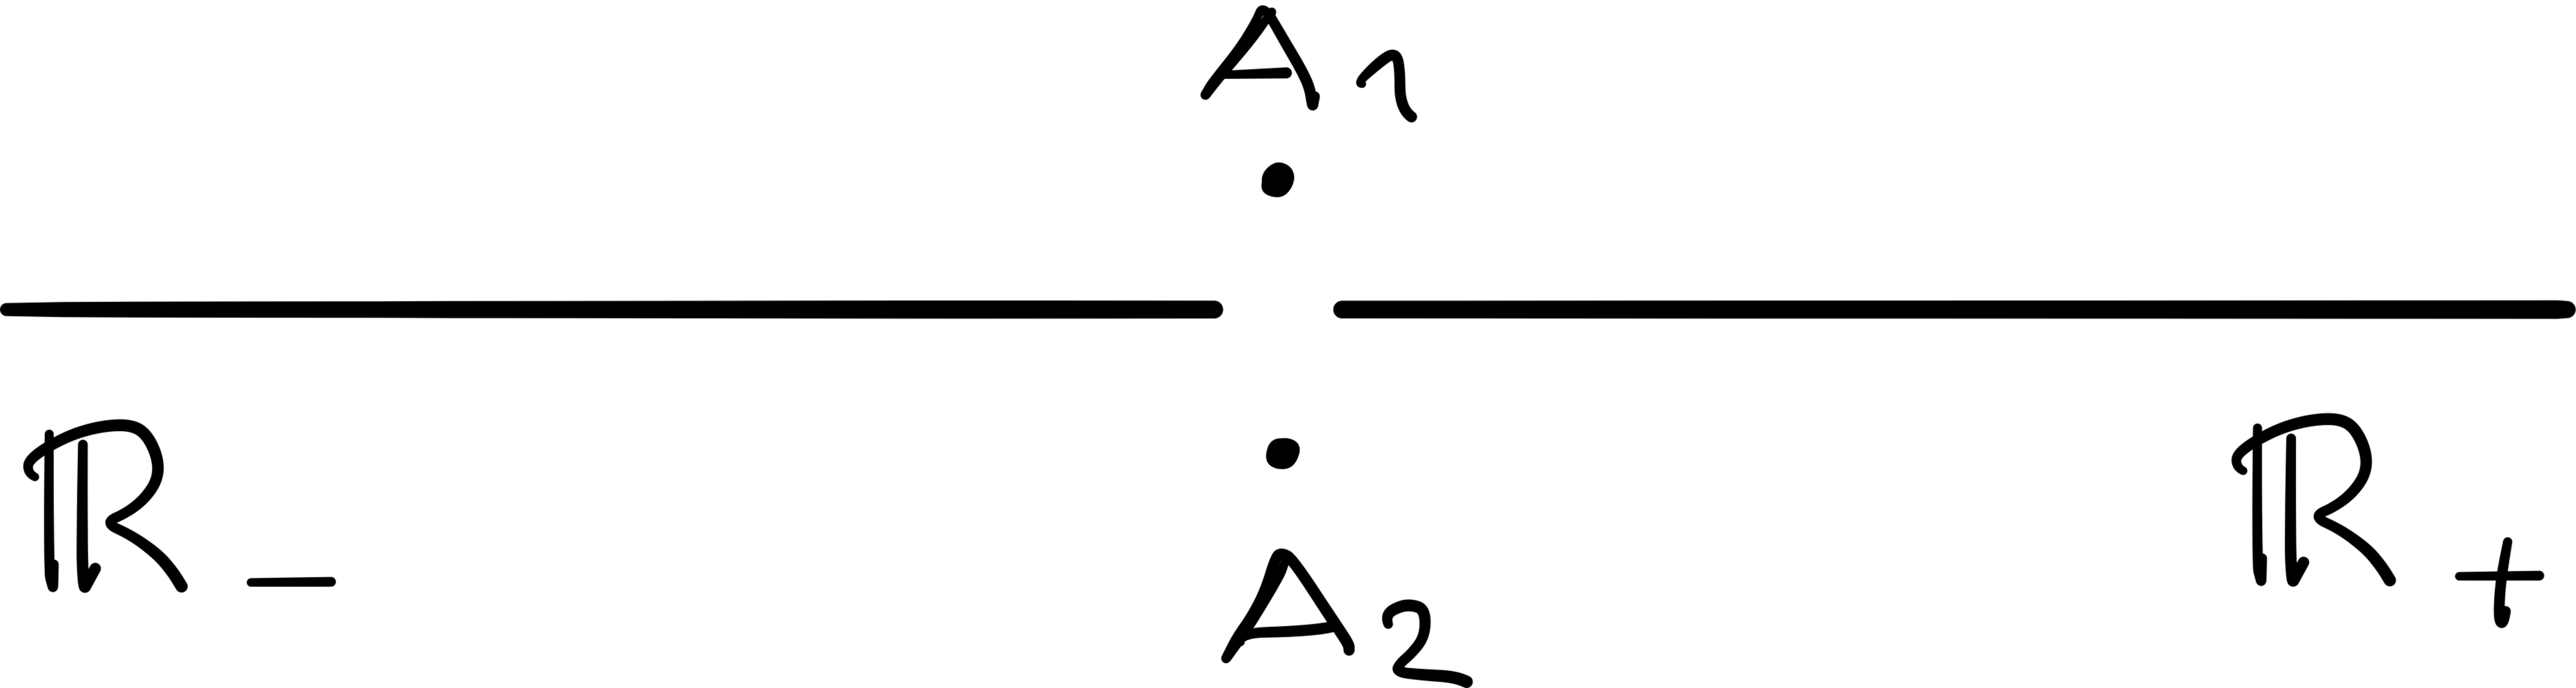
\includegraphics{1_ex_1_0_11.pdf}
    \label{fig:hausdorff-not-locally-euclidean}
    \caption{A locally euclidean space which is not Hausdorff.}
  \end{marginfigure}
  Let $A_1, A_2$ be two point not on the real line $\R$ and define $M:= (\R\setminus\{0\})\cup\{A_1,A_2\}$.
  Define the two charts
  \begin{equation}
  \phi_j:(\R\setminus\{0\})\cup\{A_j\} \to \R, \quad
  \phi_j(x) = \begin{cases} x &\mbox{if } x\neq A_j\\ 0 & \mbox{if } x = A_j \end{cases}, \quad
  j = 1,2.
  \end{equation}
  \begin{enumerate}[(a)]
    \item Show that $\phi_1$ and $\phi_2$ are homeomorphisms with respect to the induced topology\footnote{Let $(X, \cT)$ be a topological space and $f: X\to Y$ some map. The induced topology on $Y$ is \begin{equation}\cU_f := \{f^{-1}(U) \;\mid\; U\in\cT\}.\end{equation}}.
    \item Show that $M$ is locally euclidean and second countable but not Hausdorff.
  \end{enumerate}
\end{exercise}

\begin{example}\label{ex:uball}
  The \emph{closed} unit ball $D_1(0)$, where similarly as before
  \begin{equation}
    D_r(x) := \{z\in\R^n \;\mid\; d(z,x) \leq r\},
  \end{equation}
  is \emph{not} a topological manifold of dimension $n$. Can you see why? In fact, this is an example of a more general concept of \emph{manifold with boundary} that we will introduce later in Chapter~\ref{sec:mbnd}.
\end{example}

\begin{example}
	Consider the set $M := \{ x\in\R^2 \;\mid\; |x^1| = |x^2| \}$ with the topology induced by $\R^2$:
   this is \emph{not} a topological manifold.
	Since the number of connected component is invariant under homeomorphisms, open connected neighbourhoods of $(0,0)\in M$ cannot be\footnote{A drawing of $M$ is worth more than a hundred words.} holomorphically mapped to open connected sets in $\R$.
\end{example}

\marginnote{There is a caveat, the theorem holds for \emph{connected} components of a Manifold. If you consider two distinct connected components, you can indeed have different dimensions for each of them.}
\newthought{There is still an elephant in the room} in need of a comment.
In our definition of topological manifolds, we are giving for granted that the dimension of the manifold is well defined, that is, if we have two different charts, $\phi_1: U \to \R^n$ and $\phi_2: U \to \R^m$, then necessarily $m=n$. Luckily this is true! The result is called \emph{Invariance Domain Theorem} and, since its proof requires advanced concepts of algebraic topology, we will not pursue it further in the course.

\section{Differentiable manifolds}

Before entering into the details of new definitions, let's recall what will be the most important tools throughout the rest of the course.

\begin{definition}
  A map $f: U \to V$ between open sets $U\subset\R^n$ and $V\subset\R^m$ is in $C^r(U,V)$ or \emph{of class $C^r$}, if it is differentiable $r$-times.
  It is called a $C^r$-diffeomorphism\footnote{With this definition a homeomorphism is a $C^1$-diffeomorphism} if it is bijective and of class $C^r$ with inverse of class $C^r$.
  We say that $f$ is \emph{smooth}, or of class $C^\infty$, if it is of class $C^r$ for every $r \geq 1$.
\end{definition}

\begin{theorem}[Chain rule]\label{thm:chainrule}
Let $U\subset\R^n$ and $V\subset\R^k$ be open sets and $f: U \to \R^k$, $g: V\to\R^m$ two continuously differentiable functions such that $f(U)\subset V$.
Then, the following holds.
\begin{enumerate}[(i)]
  \item\label{thm:chainrule1} The function $g\circ f: U\subset\R^n \to\R^m$ is continuously differentiable and its total derivative \eqref{eq:jacobian} at a point $x\in U$ is given by
\begin{equation}
  D(g\circ f)(x) = D(g(f(x)) \circ Df(x).
\end{equation}
\item\label{thm:chainrule2} Denote $x=(x^1, \ldots, x^n)\in\R^n$ and $y=(y^2,\ldots,y^k)\in\R^k$ the coordinates on the respective euclidean spaces and $f=(f^1,\ldots,f^k)$ and $g=(g^1,\ldots,g^m)$ the components of the functions. Then the partial derivatives of $g\circ f$ are given by
\begin{equation}
  \frac{\partial g^i\circ f}{\partial x^j}(x)
  = \sum_{r=1}^k \frac{\partial g^i}{\partial y^r}(f(x)) \frac{\partial f^r}{\partial x^j}(x),
\qquad 1\leq i \leq m,\; 1\leq j\leq n.
\end{equation}
\end{enumerate}
\end{theorem}

\begin{remark}
Theorem~\ref{thm:chainrule} has some very deep consequences.
First of all \ref{thm:chainrule} \ref{thm:chainrule2} tells us that that composition preserves the regularity, that is the composition of functions  of class $C^r$ is itself a function of class $C^r$.
Second, if $f:U\subset\R^n\to V\subset\R^m$ is a diffeomorphism, then \ref{thm:chainrule} (\ref{thm:chainrule1}) implies that $n=m$.
\marginnote[-1.5em]{It follows from the fact that $Df(x)$ is an invertibe matrix and with inverse is $D(f^{-1})(f(x))$.}
\end{remark}

Since differentiability is a \emph{local} property and topological manifolds are \emph{locally} like euclidean spaces, it seems reasonable to expect that we can lift the definitions directly from $\R^n$.
If we are given a continuous map between two topological manifolds, we can locally view it as a continuous map between two Euclidean spaces.
Generalizing this further, we could conceivably say that our original map is differentiable if the local map is.

\newthought{As usual, the devil is in the details}: a topological manifold is only homeomorphic to a Euclidean space, and a different choice of homeomorphism might affect whether the local map is differentiable or not.
We need to have extra care to ensure that these lifted definitions keep making sense when we use different charts that overlap.

The solution is to introduce a little more structure to the problem.

\begin{definition}\label{def:crcomp}
We say that two charts $(U_1, \phi_1)$ and $(U_2, \phi_2)$ on a topological manifold $M$ are \emph{compatible} if either $U_1 \cap U_2 = \emptyset$ or if the \emph{transition map}\footnote{Both the composition maps $\phi_1 \circ \phi_2^{-1}$ and $\phi_2 \circ \phi_1^{-1}$ are called transition maps. Both maps are necessarily homeomorphisms since $\phi_1$ and $\phi_2$ are.}
\begin{equation}
  \phi_1 \circ \phi_2^{-1} : \phi_2(U_1\cap U_2) \to \phi_1(U_1 \cap U_2)
\end{equation}
is a smooth diffeomorphism.
\end{definition}

\begin{figure*}[htp]
  \centering
  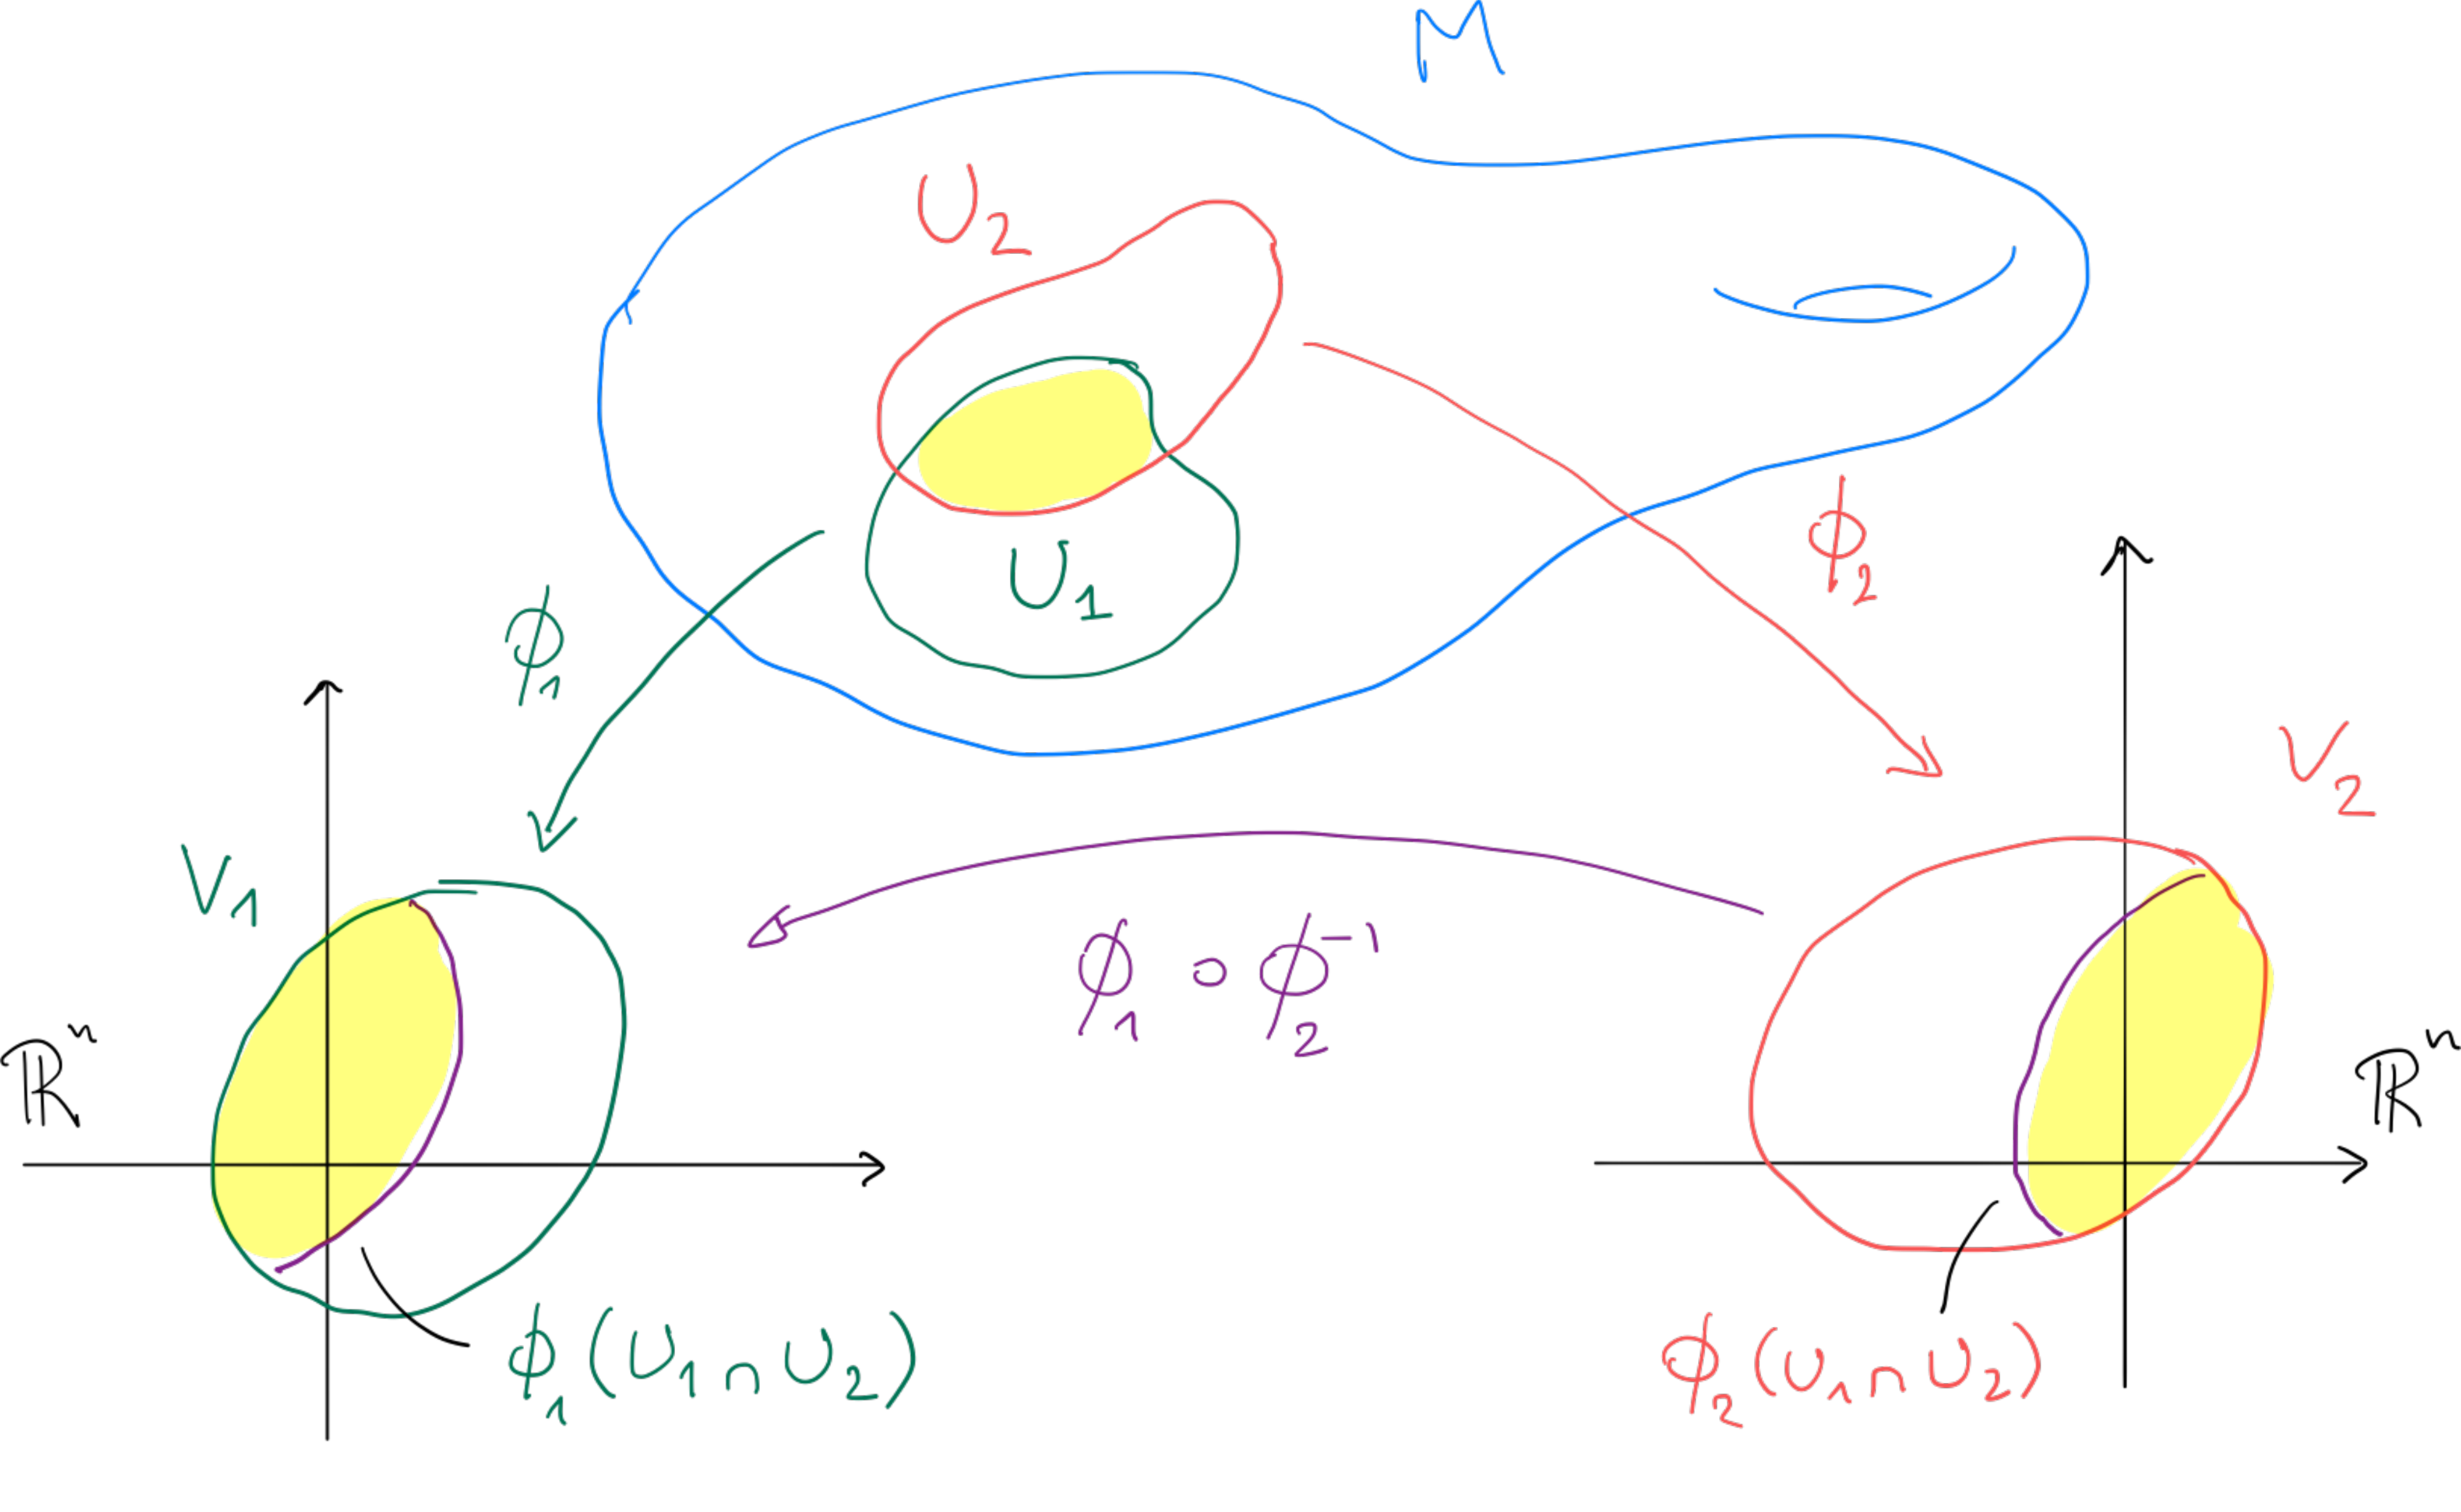
\includegraphics{1_2-compatible-charts.pdf}
  \caption{Charts are compatible if they coincide on the intersections of their coordinate neighbourhoods.}
  \label{fig:1.2-compatible-charts}
\end{figure*}

With these at hand, let's jump into the definition of smooth manifolds.

\begin{definition}\label{def:cratlas}
  A \emph{smooth atlas} is a collection
  \begin{equation}
    \cA = \{\phi_\alpha: U_\alpha \to V_\alpha \;\mid\; \alpha\in A\}
  \end{equation}
  of pairwise compatible charts that cover\footnote{I.e. such that $M = \cup_{\alpha\in A} U_\alpha$. One calls the set $\{U_\alpha \;\mid\; \alpha\in A\}$, covering $M$ with open sets, a \emph{open cover} of $M$. Here $A$ is some index set, not necessarily countable.} $M$.

  Two smooth atlases are \emph{equivalent} if their union is also a smooth atlas. That is if any two charts in the atlases are compatible.
\end{definition}

\begin{exercise}
  Show that the equivalence of atlases is really an equivalence relation.
\end{exercise}

\begin{definition}\label{def:diffstr}
  A \emph{differentiable structure}, or more precisely a \emph{smooth structure}, on a topological manifold is an equivalence class of smooth atlases.
  \marginnote{The union of all atlases in a differentiable structure is the \emph{unique} \emph{maximal} atlas in the equivalence class. There is a one-to-one correspondence between differentiable structures and maximal differentiable atlases: for convenience and to lighten the notation, from now on, we will always regard a differentiable structure as a differentiable maximal atlas without further comments.}
\end{definition}

\begin{notation}
By a \emph{chart $(U, \phi)$ about $p$} in a manifold $M$ we mean a chart in the differentiable structure of $M$ such that $p\in U$.
\end{notation}

\begin{definition}\label{def:diffmanifold}
  A \emph{smooth manifold} of dimension $n$ is a pair $(M, \cA)$ of a topological $n$-manifold $M$ and a smooth structure $\cA$ on $M$.
  \marginnote[1em]{There are no preferred coordinate charts on a manifold: all coordinate systems compatible with the differentiable structure are on equal footing.}
\end{definition}

In colloquial language, a differentiable manifold is a space covered by charts with differentiable transition maps.

Whenever possible we will omit the differentiable structure $\cA$ from the notation and just write $M$.
We may write $M^n$ when we want to emphasize the dimension $n$ of $M$.

\begin{exercise}
  Show that on a second countable differentiable manifold it is always possible to find a countable atlas.
\end{exercise}

\begin{exercise}\label{exe:subsetsmanifolds}
  $\R^n$ with the \emph{standard} smooth structure $\cA=(\R^n, \id_{\R^n})$ is trivially a smooth manifold of dimension $n$.

  In fact, any open subset $U\subset\R^n$ can be made into a smooth manifold in a natural way: pick the atlas $\cA=(U, \id_{\R^n}|_U)$.

  In the same way, any open subset $U$ of a smooth manifold $M$ is a smooth manifold.
  Which atlas would you choose?

  More generally, if $V$ is any $n$-dimensional real vector space, then the standard smooth structure on $V$ is the one induced by the smooth atlas consisting of a single chart $(V, T)$ where $T: V \to R^n$ is some linear isomorphism.
  Why is this independent of the choice of the isomorphism $T$?

  This example has a very interesting consequence.
  The space $\mathrm{Mat}(n)$ of $n\times n$-matrices can be identified with $\R^{n^2}$ by writing the elements of the matrix as a $n^2$-vector.
  This gives to $\mathrm{Mat}(n)$ a structure of differentiable manifold.
  The subset of invertible matrices $GL(n) = \{ A \in \mathrm{Mat}(n) \;\mid\; \det A \neq 0\}$, widely known as the \emph{general linear group}, being an open subset of $\mathrm{Mat}(n)$ (why?) is itself a differentiable manifold.
Can you guess if such manifold is connected or not?
\end{exercise}

\begin{notation}\label{ntn:coords}
  We will stick to the notation of \cite{book:tu}.
  In the context of manifolds, denote $r^i: \R^n\to\R$, $1\leq i\leq n$, the standard coordinates on $\R^n$. With this notation, if $e_i$ denotes the $i$th standard basis vector in $\R^n$, then $r^i(e_j) = \delta^i_j$.
  \marginnote[-1em]{The Kronecker delta $\delta_j^i$ is defined by $\delta_j^i = 1$ if $i=j$ and $\delta_j^i = 0$ otherwise.}

  If $(U, \phi:U\to\R^n)$ is a chart of a manifolds, then $x^i = r^i\circ\phi$ will denote the $i$-th component of $\phi$ and denote $\phi = (x^1, \ldots, x^n)$ and, when convenient, $(U,\phi) = (U, x^1, \ldots, x^n)$.

  Thus, for $p\in U$, $(x^1(p), \ldots, x^n(p))$ is a point\footnote{By abuse of notation we sometimes omit the $p$! Thus $(x^1, \ldots, x^n)$ can stand either for local coordinates or a point in $\R^n$: which one it is should be clear from the context.} in $\R^n$. The functions $x^1, \ldots, x^n$  are called \emph{(local) coordinates} on $U$.
\end{notation}

An advantage of this new notation is that we can talk about coordinates without the need to explicitly reference charts. In other words, we can say
\begin{quote}
  Let $p\in M$ and choose local coordinates $(x^1, \ldots, x^n)$ about $p$...
\end{quote}
or even
\begin{quote}
  Let $x=(x^1, \ldots, x^n)\in M$ be a point in $M$...
\end{quote}
dropping the distinction between $p$ and $x$, both in place of
\begin{quote}
  Let $p \in M$ and $(U, \phi)$ a chart defined on a neighbourhood $U$ of $p$.
  Let $x^i = r^i \circ\phi$ denote the components of $\phi$ with respect to the standard euclidean coordinates...
\end{quote}

\begin{example}\label{ex:S1emb}
  The unit circle
  \begin{equation}
    \bS^1 := \{x\in\R^2 \;\mid\; \|x\|=1\}\subset\R^2
  \end{equation}
  with the relative topology\footnote{Let $(X,\cT)$ be a topological space and $Y\subset X$. The relative topology on $Y$ is \begin{equation}\mathcal{V}:=\{V\subset Y\;\mid\;\exists U\in\cT \mbox{ s.t. } V = U \cap Y\}.\end{equation}} is a $1$-dimensional topological manifold.
  To provide the local homeomorphisms to $\R^n$ and define a smooth structure four $\bS^1$ it is enough to define the following four charts:
  \begin{equation}
    \begin{aligned}
      &V_1 := \{ x^1 > 0 \},\quad \phi_1: V_1 \to (-1, 1), \quad \phi_1(x) := x^2,\\
      &V_2 := \{ x^1 < 0 \},\quad \phi_2: V_2 \to (-1, 1), \quad \phi_2(x) := x^2,\\
      &V_3 := \{ x^2 > 0 \},\quad \phi_3: V_3 \to (-1, 1), \quad \phi_3(x) := x^1,\\
      &V_4 := \{ x^2 < 0 \},\quad \phi_4: V_4 \to (-1, 1), \quad \phi_4(x) := x^1.
    \end{aligned}
  \end{equation}
  What do these charts look like?
\end{example}

\begin{exercise}
  Let $f: \R^n \to \R^m$ be a smooth map.
  Show that its graph
  \begin{equation}
    \Gamma_f := \{(x, f(x)) \;\mid\; x\in\R^n\} \subset\R^{n+k}
  \end{equation}
  is a smooth manifold of dimension $n$.
\end{exercise}

\begin{example}
  The definition of smooth manifold does not require $M$ to be embedded into some ambient space as in the examples above.
  In fact, we can define the differentiable manifold $\bS^1$ by equipping the topological quotient space $\R/\Z$ with the two charts
  \begin{equation}\textstyle
    \phi_1 : \R/\Z \setminus\{[0]\} \to (0,1)
    \quad\mbox{and}\quad
    \phi_2 : \R/\Z \setminus\{[\frac12]\} \to (-\frac12,\frac12)
  \end{equation}
  which map $[x]\in\R/\Z$ to its representation in $(0,1)$ or $[-\frac12, \frac12)$ respectively.
  The manifold obtained in this way is diffeomorphic to the one defined in Example \ref{ex:S1emb}.
\end{example}

\begin{example}[Product manifolds]
Given two manifolds $(M_1, \cA_1)$ and $(M_2, \cA_2)$, we can define the \emph{product manifold} $M_1 \times M_2$ by equipping $M_1 \times M_2$ with the product topology\footnote{Open sets in the product are products of open sets from the respective topological spaces.} and cover the space with the atlas $\{ (U_1\times U_2, (\phi_1, \phi_2)) \;\mid\; (U_1, \phi_1)\in\cA_1, (U_2, \phi_2)\in \cA_2\}$.
\end{example}

Note that smooth manifolds do not yet have a metric structure: distances between the points are not defined.
However, they are \emph{metrizable}\footnote{This property is far more general: all the topological manifolds are metrizable.}: there exists some metric on the manifold that induces the given topology on it.
This allows to always view manifolds as metric spaces.

\begin{remark}
	There exist examples of topological manifolds without smooth structures.
	It is also known that smooth manifolds of dimension $n < 4$ have exactly one smooth structure while ones of dimension $n > 4$ have finitely many\footnote{A beautiful example of this is the $7$-sphere $\bS^7$ which is known to have 28 non-diffeomorphic smooth structures.}.
	The case $n = 4$ is unknown: if you prove that there is only one smooth structure, you will have shown the smooth Poincar\'e conjecture.
\end{remark}

Instead of always constructing a topological manifold and then specify a smooth structure, it is often convenient to combine these steps into a single construction.
This is especially useful when the initial set is not equipped with a topology.
In this respect, the following lemma provides a welcome shortcut: in brief it says that given a set with suitable ``charts'' that overlap smoothly, we can use the charts to define both a topology and a smooth structure on the set.

\begin{lemma}[Smooth manifold lemma]\label{lem:manifold_chart}
  Let $M$ be a set. Assume that we are given a collection $\{U_\alpha\mid \alpha\in A\}$ of subsets of $M$ together with bijections $\phi_\alpha: U_\alpha\to\phi(U_\alpha)\subseteq\R^n$, where $\phi(U_\alpha)$ is an open subset of $\R^n$. Assume in addition that the following hold:
  \begin{enumerate}
    \item For each $\alpha, \beta \in A$, the sets $\phi_\alpha(U_\alpha \cap U_\beta)$ and $\phi_\beta(U_\alpha \cap U_\beta)$ are open in $\R^n$.
    \item If $U_\alpha \cap U_\beta \neq 0$, the map $\phi_\beta\circ\phi_\alpha^{-1}: \phi_\alpha(U_\alpha \cap U_\beta)\to \phi_\beta(U_\alpha \cap U_\beta)$ is smooth.
    \item Countably many of the sets $U_\alpha$ cover $M$.
    \item If $p\neq q$ are points in $M$, either there exists $\alpha$ such that $p,q\in U_\alpha$ or there exists $\alpha,\beta$ with $U_\alpha\cap U_\beta=\emptyset$ such that $p\in U_\alpha$ and $q\in U_\beta$.
  \end{enumerate}
  Then $M$ has a unique smooth manifold structure such that each $(U_\alpha,\phi_\alpha)$ is a smooth chart.
\end{lemma}
\begin{exercise}
  Prove Lemma~\ref{lem:manifold_chart}. Hint: declare all the $\phi_\alpha$ to be homeomorphisms and use the hypotheses to check the definition of a smooth manifold.
\end{exercise}

\begin{example}[Grassmannian (Manifold)]
  \todo{Lee, Example 1.36}
\end{example}

\begin{tcolorbox}
  The general definition of $C^r$-manifolds is mostly a matter of replacing occurrences of ``smooth'' in the text with $C^r$.
  The study of these more general structures is not dissimilar from what we will see in this course, with the exception of analytic and $C^0$-manifolds, but it introduces an unnecessary extra level of verbosity.
  In these notes we will only deal with smooth manifolds.
\end{tcolorbox}

\section{Intermission: exercises}
\TODO

\section{Smooth maps and differentiability}

With a well defined differentiable structure and the idea of compatible charts, we have all the ingredients to lift the definition of differentiable maps from the euclidean world.

Before considering the general definition of a differentiable map, let's look at the simpler example of differentiable functions $f:M\to\R$ between a smooth manifold $M$ and $\R$.

\begin{definition}
  A function $f:M\to\R$ from a smooth manifold $M$ of dimension $n$ to $\R$ is \emph{smooth}, or \emph{of class $C^\infty$}, if for any chart $(\phi, V)$ of $M$ the map $f\circ\phi^{-1}:\phi(V)\subset\R^n \to \R$ is smooth as a euclidean function.
  \begin{marginfigure}
    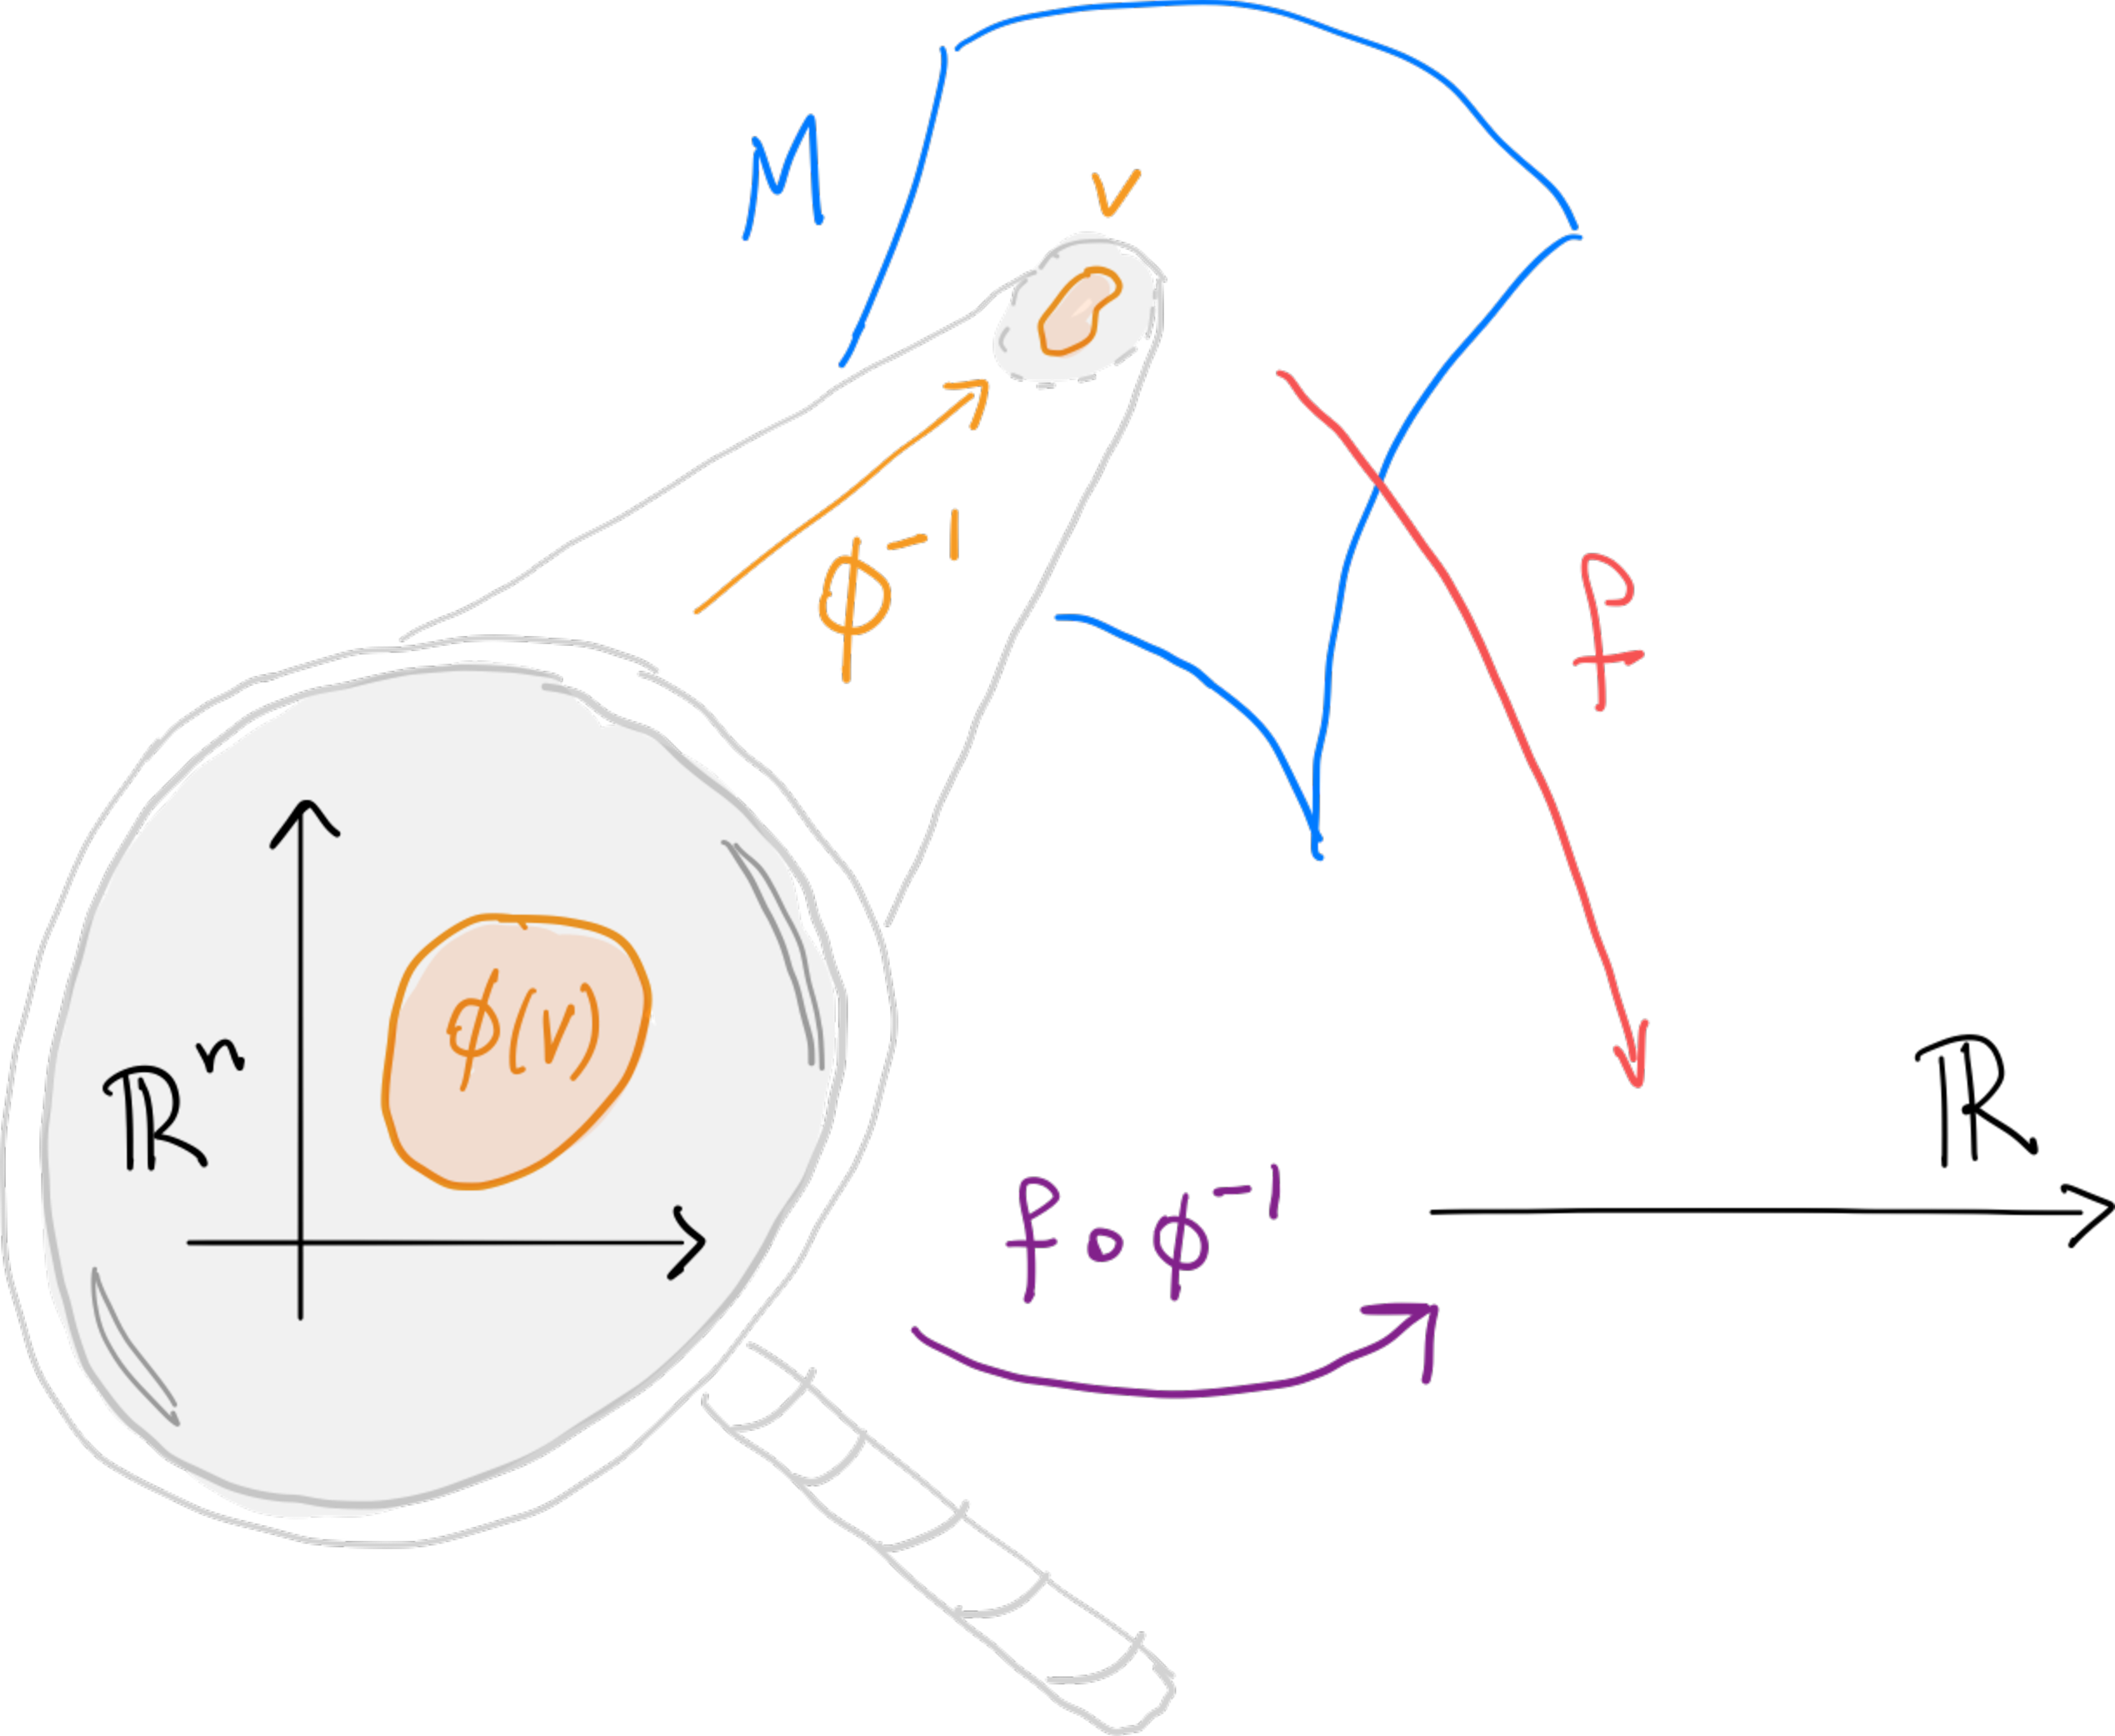
\includegraphics{1_5-diff-fun-v2.pdf}
    \label{fig:diff-fun}
    \caption{A function is differentiable if it is differentiable as a euclidean function through the magnifying lens provided by the charts.}
  \end{marginfigure}
  We denote the space of smooth functions by $C^\infty(M)$.
\end{definition}

This, colloquially speaking, means that a function is differentiable if it is differentiable as a euclidean function through the magnifying lens (see Figure~\ref{fig:diff-fun}) provided by the charts.

\begin{exercise}
  Define on the following operations.
  For any $f,g\in C^\infty(M)$, $c\in\R$,
  \begin{equation}
    (f+g)(x) := f(x) + g(x),\quad
    (fg)(x) := f(x) g(x),\quad
    (cf)(x) := c f(x).
  \end{equation}
  Then, the space $C^\infty(M)$ endowed with the operations above is an \emph{algebra}\footnote{I.e. a vector space where you can also multiply two elements.} over $\R$.
\end{exercise}

Which immediately gives away the general definition.

\begin{definition}
  Let $F:M_1\to M_2$ be a continuous map \footnote{Remember: continuity is not a problem since $M_1$ and $M_2$ are topological spaces.} between two smooth manifolds of dimension $n_1$ and $n_2$ respectively.
  We say that $f$ is \emph{smooth}, or \emph{of class $C^\infty$}, if, for any chart $(\phi_1, V_1)$ of $M_1$ and $(\phi_2, V_2)$ of $M_2$, the map
  \begin{align}
    \phi_2 \circ F \circ \phi_1^{-1}: U_1 \to U_2,\\
    U_1 := \phi_1(V_1 \cap f^{-1}(V_2))\subset\R^{n_1},\\
    U_2 := \phi_2(f(V_1) \cap V_2)\subset\R^{n_2},
  \end{align}
  is smooth as a euclidean function.
  \marginnote[-6em]{Differently from your calculus classes, we are defining differentiability \emph{before} we define what the derivative is. Getting to it will require some amount of work, and will have to wait until the next chapter.}

  We denote by $C^\infty(M_1, M_2)$ the set of all functions $F:M_1\to M_2$ of class $C^\infty$.

  The map $\hat F := \phi_2 \circ F \circ \phi_1^{-1}$ is called the \emph{coordinate representation of $F$} with respect to the given coordinates.
\end{definition}

\begin{figure}[htp]
  \centering
  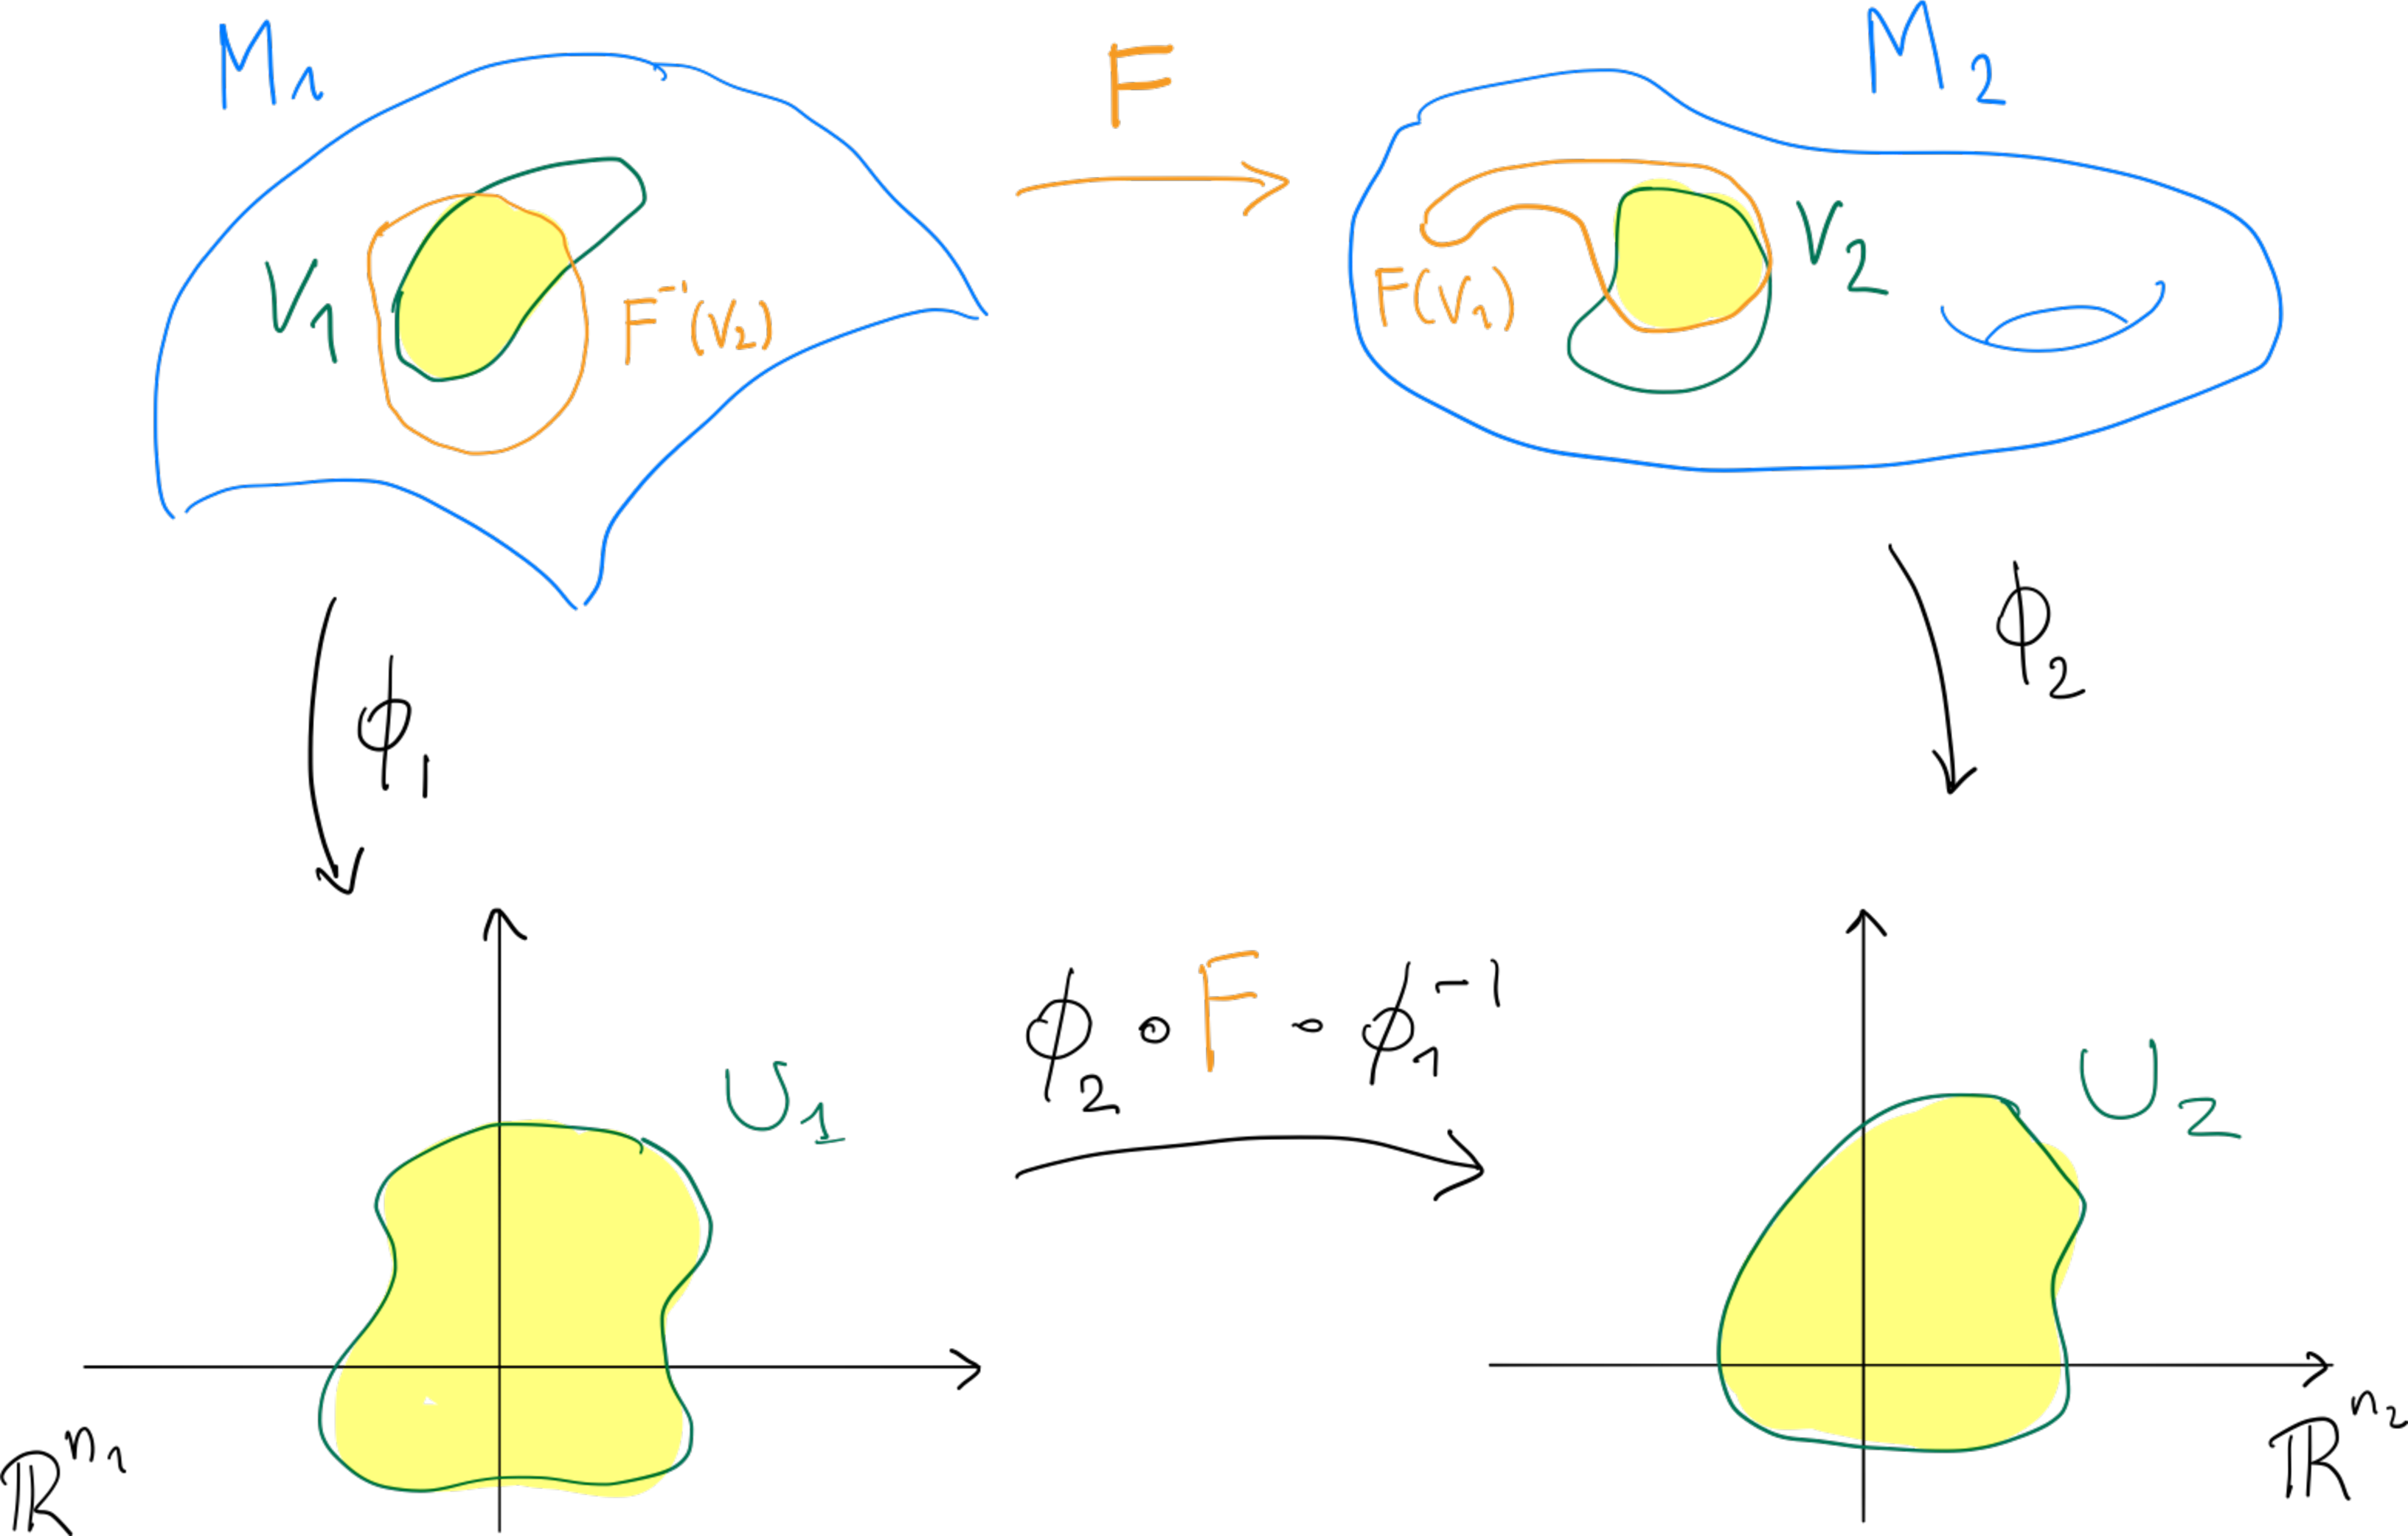
\includegraphics{1_3-diffble_maps.pdf}
  \caption{Maps are differentiable when they are differentiable as maps between euclidean spaces.}
  \label{fig:1.3-differentiable_maps}
\end{figure}

A first observation about our definition of smooth maps is that as one would hope, smooth imply continuity.

\begin{exercise}
  Shoa that every smooth map is continuous.
\end{exercise}

\begin{definition}
A \emph{diffeomorphism} $F$ between two smooth manifolds $M_1$ and $M_2$ is a bijective map such that $F\in C^\infty(M_1, M_2)$ and $F^{-1}\in C^\infty(M_2, M_1)$.

Two smooth manifolds $M_1$ and $M_2$ are called \emph{diffeomporphic} if there exists a diffeomorphism $F:M_1\to M_2$ between them.
\end{definition}

\begin{example}
Any chart $(V, \phi)$ of a manifold $M$ is a diffeomorphism between the manifolds $V\subset M$ and $\phi(V)\subset\R^n$.
\end{example}

\begin{exercise}
  Prove the following propositions and aid your reasoning by drawing the relevant figures.
  \begin{proposition}
    Let $M$ be a smooth manifold of dimension $n$.
    Then $F:M\to\R^m$ is smooth iff for all charts $(U,\phi)$ of $M$, the function $F\circ\phi^{-1}:\phi(U)\to\R^m$ is smooth.
  \end{proposition}
  \begin{proposition}
    Let $M$ be a smooth manifold of dimension $n$.
    Then $f:\R^m\to M$ is smooth iff for all charts $(U,\phi)$ of $M$, the function $\phi\circ F:F^{-1}(U)\to\R^m$ is smooth.
  \end{proposition}
  \begin{proposition}
    Let $M, N, P$ be three smooth manifolds, and suppose that $F:M\to N$ and $G:N\to P$ are smooth.
    Then $G\circ F\in C^\infty(M, P)$.
  \end{proposition}
  \marginnote{In Proposition~\ref{prop:uniqdiffeoinclusion} it is not enough to ask that $\iota$ is smooth! As counterexample consider the two manifolds $(\R, \cA_1)$ with $\cA_1 := \{(\R, \id_\R)\}$ and $(\R, \cA_2)$ with $\cA_2 := \{(\R, x\mapsto x^3)\}$. The inclusion of open sets in $\R$ is smooth in both cases but is a diffeomorphism only in one.}
  \begin{proposition}\label{prop:uniqdiffeoinclusion}
    Let $M$ be a manifold and $U\subset M$ an open set.
    Then $U$ has a unique differentiable structure such that the inclusion $\iota:U\hookrightarrow M$ is a diffeomorphism.
  \end{proposition}
  \begin{proposition}[Smoothness is a local property]\label{prop:smoothlocal}
    Let $F:M\to N$ be a continuous function and let $\{U_i\}_{i\in I}$ be an open cover for $M$. Then $F|_{U_i}:U_i \to N$ is smooth for every $i\in I$ iff $F:M\to N$ is smooth.
  \end{proposition}
\end{exercise}

The following corollary is just a restatement of Proposition~\ref{prop:smoothlocal}, but provides a useful perspective on the construction of smooth maps.

\begin{proposition}[Gluing lemma for smooth maps]
  Let $M$ and $N$ be two smooth manifolds and let $\{U_\alpha\mid\alpha\in A\}$ be an open cover of $M$.
  Suppose that for each $\alpha\in A$ we are given a smooth map $F_
  \alpha:U_\alpha\to N$ such that the maps agree on the overlaps: $F_\alpha|_{U_\alpha\cap U_\beta} = F_\beta|_{U_\alpha\cap U_\beta}$ for all $\alpha,\beta\in A$. 
  Then there exists a unique smooth map $F:M\to N$ such that $F|_{U_\alpha} = F_\alpha$ for each $\alpha\in A$.
\end{proposition}

\begin{tcolorbox}
From now on, when we write manifold, chart, atlas, etc. we always mean smooth manifold, smooth chart, smooth atlas, etc..
\end{tcolorbox}

\section{Partitions of unity}

\newthought{Cutoff functions} are a class of smooth functions that will be of crucial importance throughout the course, and whose existence cannot be given for granted.
Since their definition and construction does not require more than what we have just seen, let's talk about them now.

First of all, recall that the \emph{support} of a smooth function $f: M \to \R$, denoted by $\supp(f)$, is defined as
\marginnote[2em]{The bar over the set denotes its closure.}
\begin{equation}
  \supp(f) := \overline{\{ p\in M \;\mid\; f(p) \neq 0\}}.
\end{equation}

We will introduce those functions with a proposition, and will spend the rest of this chapter proving it.

\begin{figure}[htp!]
  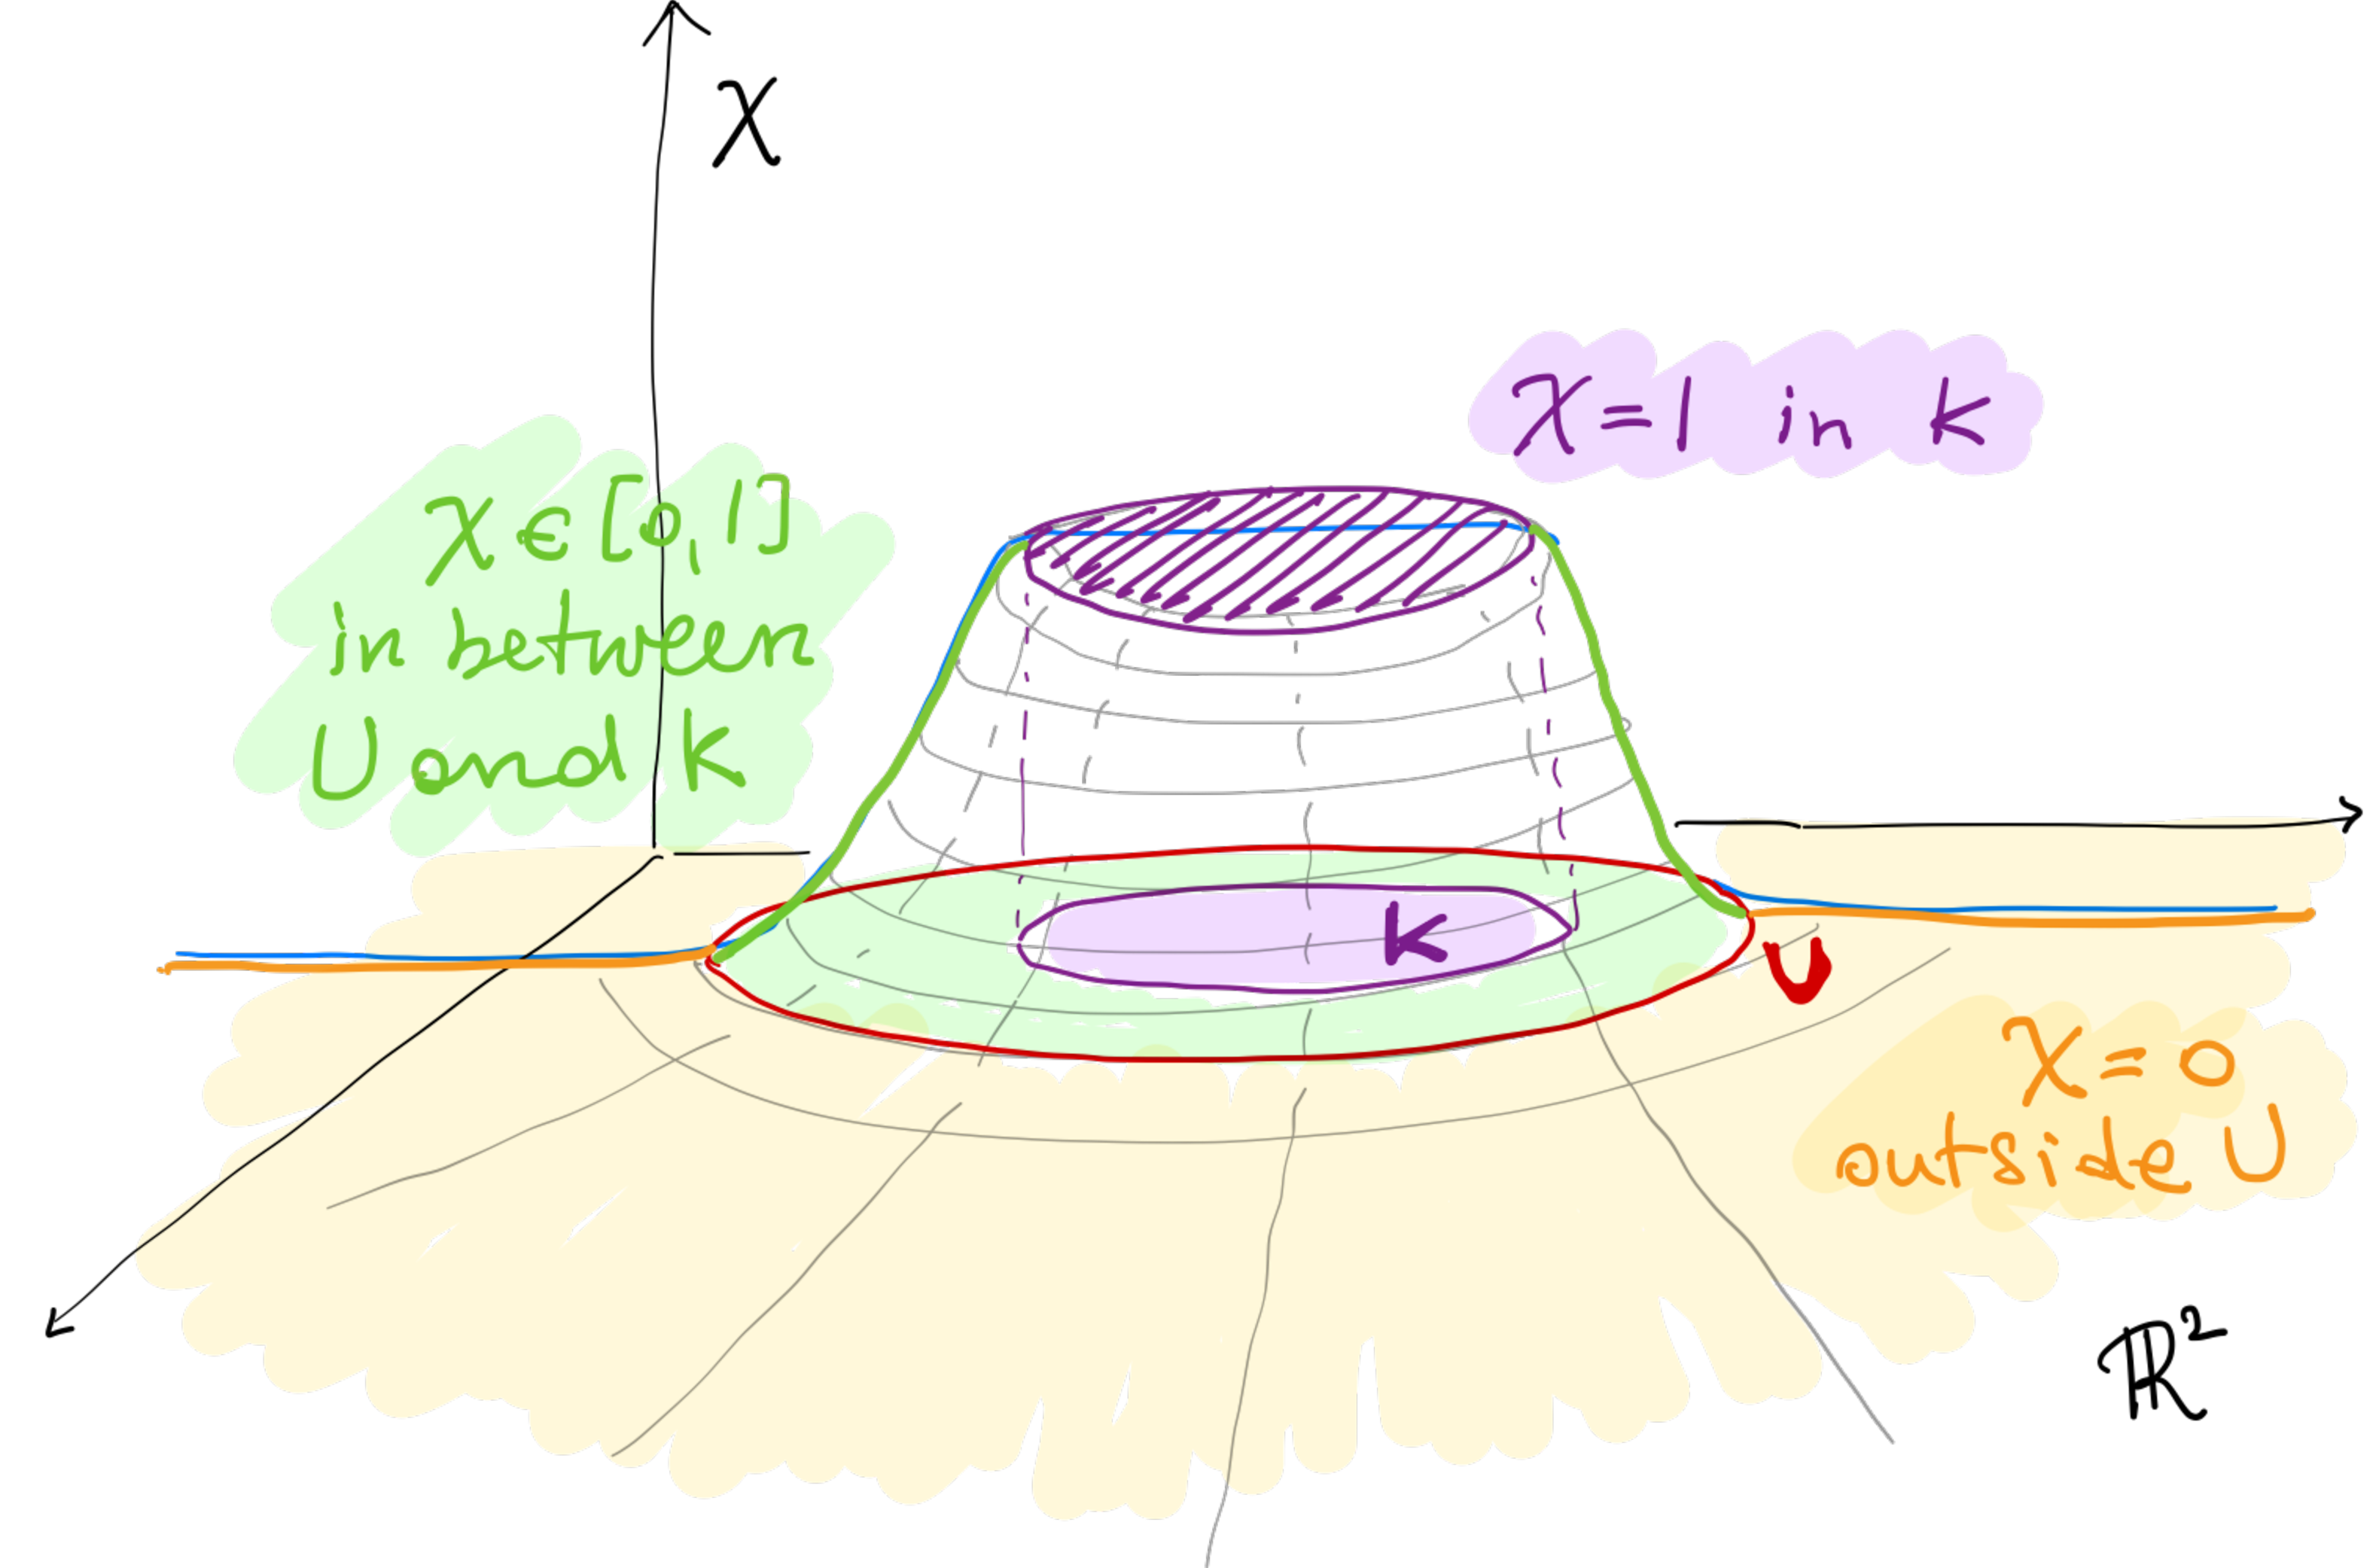
\includegraphics{1_6-cutoffs.pdf}
\end{figure}

\begin{proposition}[Cutoff functions]\label{prop:cutoff}
  Let $M$ be a smooth manifold and $K\subset U\subset M$ two subsets such that $K$ is closed and $U$ is open.
  Then, there exists a smooth function $\chi: M \to\R$, called \emph{cutoff} function, with the following properties
  \begin{enumerate}
    \item $0 \leq \chi \leq 1$ for all $p\in M$;
    \item $\supp(\chi)\subset U$;
    \item $\chi(p) = 1$ for all $p\in K$.
  \end{enumerate}
\end{proposition}

The proof of this proposition involves a general result which is quite technical and whose proof will be omitted.
You can refer to \cite{book:lee, book:tu} if you are curious to see the details.

Instead, we will show a special case of Proposition~\ref{prop:cutoff}. The main reason is that it involves an explicit construction of the cutoff which can be convenient to have at hand later on.

\begin{lemma}[Cutoff functions, compact case]
  Let $M$ be a smooth manifold and $K\subset U\subset M$ two subsets such that $K$ is compact and $U$ is open.
  Then, there exists a smooth function $\chi: M \to\R$ with the following properties
  \begin{enumerate}
    \item $0 \leq \chi \leq 1$ for all $p\in M$;
    \item $\supp(\chi)\subset U$;
    \item $\chi(p) = 1$ for all $p\in K$.
  \end{enumerate}
\end{lemma}
\begin{proof}
  \newthought{Part 1}.
  To warm up, let's do some first year analysis.
  For any pair of real numbers $r < R$ there exists a smooth function $f: \R \to [0,1]$ such that $f(t) = 1$ for $t \leq r$, $f(t) = 0$ for $t \geq R$ and $0<f(t)<1$ for $t\in(r,R)$.
  
  We can construct this explicitly by means of the function
  \begin{equation}
    h:\R\to\R, \quad h(t):= \begin{cases}
      e^{-1/t}, & t>0,\\
      0, & t \leq 0.
    \end{cases}
  \end{equation}

  \begin{exercise}
    Prove by induction that for $t>0$ and $k\geq 0$, the $k$th derivative $f^{(k)}(t)$ is of the form $p_{2k}(1/t)e^{-1/t}$ for some polynomial $p_{2k}(x)$ of degree $2k$ in $x$.
    Use this to show that $f\in C^\infty(\R)$ and that $f^{(k)}(0) = 0$ for all $k\geq 0$.
  \end{exercise}

  The function $f$ that we are seeking is then\footnote{Exercise: check that such function $f$ satisfies all the desired properties.} given by
  \begin{equation}
    f(t) := \frac{h(R-t)}{h(R-t) + h(t-r)}.
  \end{equation}

  \newthought{Part 2}.
  Let's extend $f$ to $\R^n$.
  Denote $B_r \subset \R^n$ the open ball of radius $r$ around the origin.
  Then, for any $0 < r < R$ we seek a function $g:\R^n\to\R$ such that $g(x) = 1$ for all $x\in \overline{B_r}$, $g(x) = 0$ for all $x\in \R^n\setminus B_R$ and $0< g(x)< 1$ for all $x\in B_R\setminus\overline{B_r}$.
  This is immediately achieved by defining $g(x) := f(\|x\|)$, where $f$ is the function defined in the previous step.

  \newthought{Part 3}.
  Let's now pick a point $p\in M$ and an arbitrary neighbourhood $U$ of $p$. Choosing an appropriate chart about $p$, the previous step implies that we can choose a smaller neighbourhood $V\subset U$ of $p$ with $\overline V\subset U$ and such that there exists a smooth function $\chi: M \to [0,1]$ satisfying $\chi(p) = 1$ for all $p\in\overline{V}$ and $\chi(p) = 0$ for all $p\in M\setminus U$.
  
  \newthought{Part 4}.
  We are ready to complete the proof.
  For each point $p\in K$, choose two neighbourhoods $V_p \subset U_p$ such that $\overline{V_p}\subset K$ and $U_p \subset U$.
  Since $K$ is compact, it admits a finite cover in terms of these sets: i.e. there are finitely many points $p_1, \ldots, p_N \in K$ such that $K \subset \bigcup_{i=1}^N V_{p_i}$.
  For each $i$, choose $\chi_i: M \to [0,1]$ as in the previous step: $\chi_i(p) = 1$ for all $p\in\overline{V_{p_i}}$ and $\chi_i(p) = 0$ for all $p\in M\setminus U_{p_i}$.
  The proof is completed by defining
  \begin{equation}
    \chi := 1 - \prod_{i=1}^N(1 - \chi_i(p)).
  \end{equation}
\end{proof}

To extend this result and prove will still require hard work and a new tool, that will be useful throughout the course an in many courses to come.

\begin{definition}
  Let $M$ be a smooth manifold. A \emph{partition of unity} is a collection $\{\rho_\alpha \mid \alpha\in A\}$ of functions $\rho_\alpha:M\to\R$ such that
  \begin{enumerate}
    \item $0 \leq \rho_\alpha \leq 1$ for all $p\in M$ and $\alpha\in A$;
    \item\label{def:pou.2} the collection $\{\rho_\alpha \mid \alpha\in A\}$ is \emph{locally finite}, that is, for any $p\in M$ there are at most finitely many $\alpha\in A$ such that $p\in\supp(\rho_\alpha)$;
    \item for all $p\in M$ one has $\sum_{\alpha\in A} \rho_\alpha(p) = 1$.
    \marginnote{For any $p$, $\sum_{\alpha\in A} \rho_\alpha(p)$ is a finite sum by \ref{def:pou.2}. Thus, the function defined by the sum $\rho := \sum \rho_\alpha$ is a well define smooth function on $M$. We call such sum a \emph{locally finite} sum.}
  \end{enumerate}
\end{definition}

\begin{remark}
Note that the existence of a partition of unity is a distinguished feature of differentiable manifolds: stronger structures, like analytic or holomorphic ones, in general fail to have one.
\end{remark}

Throughout the course we will be mostly interested in partitions of unity $\{\rho_\alpha \mid \alpha\in A\}$ which are \emph{subordinate} to an open cover $\{U_\alpha\mid\alpha\in A\}$, that is, such that $\supp_\alpha(\rho_\alpha) \subset U_\alpha$ for each $\alpha\in A$.

\begin{theorem}\label{thm:partitionof1}
  Let $M$ be a smooth manifold. For any open cover $\{U_\alpha\mid\alpha\in A\}$ of $M$, there exists a partition of unity $\{\rho_\alpha \mid \alpha\in A\}$ subordinate to $\{U_\alpha\mid\alpha\in A\}$.
\end{theorem}

With this result at hand, Proposition~\ref{prop:cutoff} can be shown very easily.

\begin{proof}[Proof of Proposition~\ref{prop:cutoff}.]
  Consider the open cover of $M$ given by $\cC:=\{M\setminus K, U\}$.
  Then Theorem~\ref{thm:partitionof1} implies that there exists a partition of unity $\{\rho_U, \rho_{M\setminus K}\}$ adapted to $\cC$. The function $\chi := \rho_U$ is our cutoff function.
\end{proof}

\section{Manifolds with boundary}\label{sec:mbnd}

\newthought{The definition of manifolds has a serious limitation}, even though it is perfectly good to describe curves\footnote{E.g. the circle seen in Example~\ref{ex:S1emb}.} and surfaces\footnote{E.g. the $n$-spheres $\bS^n$ in the homework sheet.}, it fails to describe many natural objects like a \emph{closed} interval $[a,b]\in\R$ or the \emph{closed} disk $D_1(0)$ of Example~\ref{ex:uball}.

Note that in both these cases, both the interior and the boundary are smooth manifolds and their dimension differ by one\footnote{In the first case the interior $(a,b)$ is a $1$-manifold and the boundary, the set $\partial[a,b] = \{a,b\}$, is a $0$-manifold. In the second case the interior of $D_1(0)$ is the open unit ball, a $2$-manifold, and the boundary $\partial D_1(0)$ is the $1$-manifold $\bS^1$.}.

Let's do a step back and think about topological manifolds: since both the closed interval and the closed disk are closed sets, we have problems to make them locally euclidean in neighbourhoods of their boundaries.
Can we modify our local model to resemble something with a boundary?

Of course this is a rhetorical question.
We can generalize our definition by considering the \emph{closed upper half-spaces}
\begin{marginfigure}[2em]
  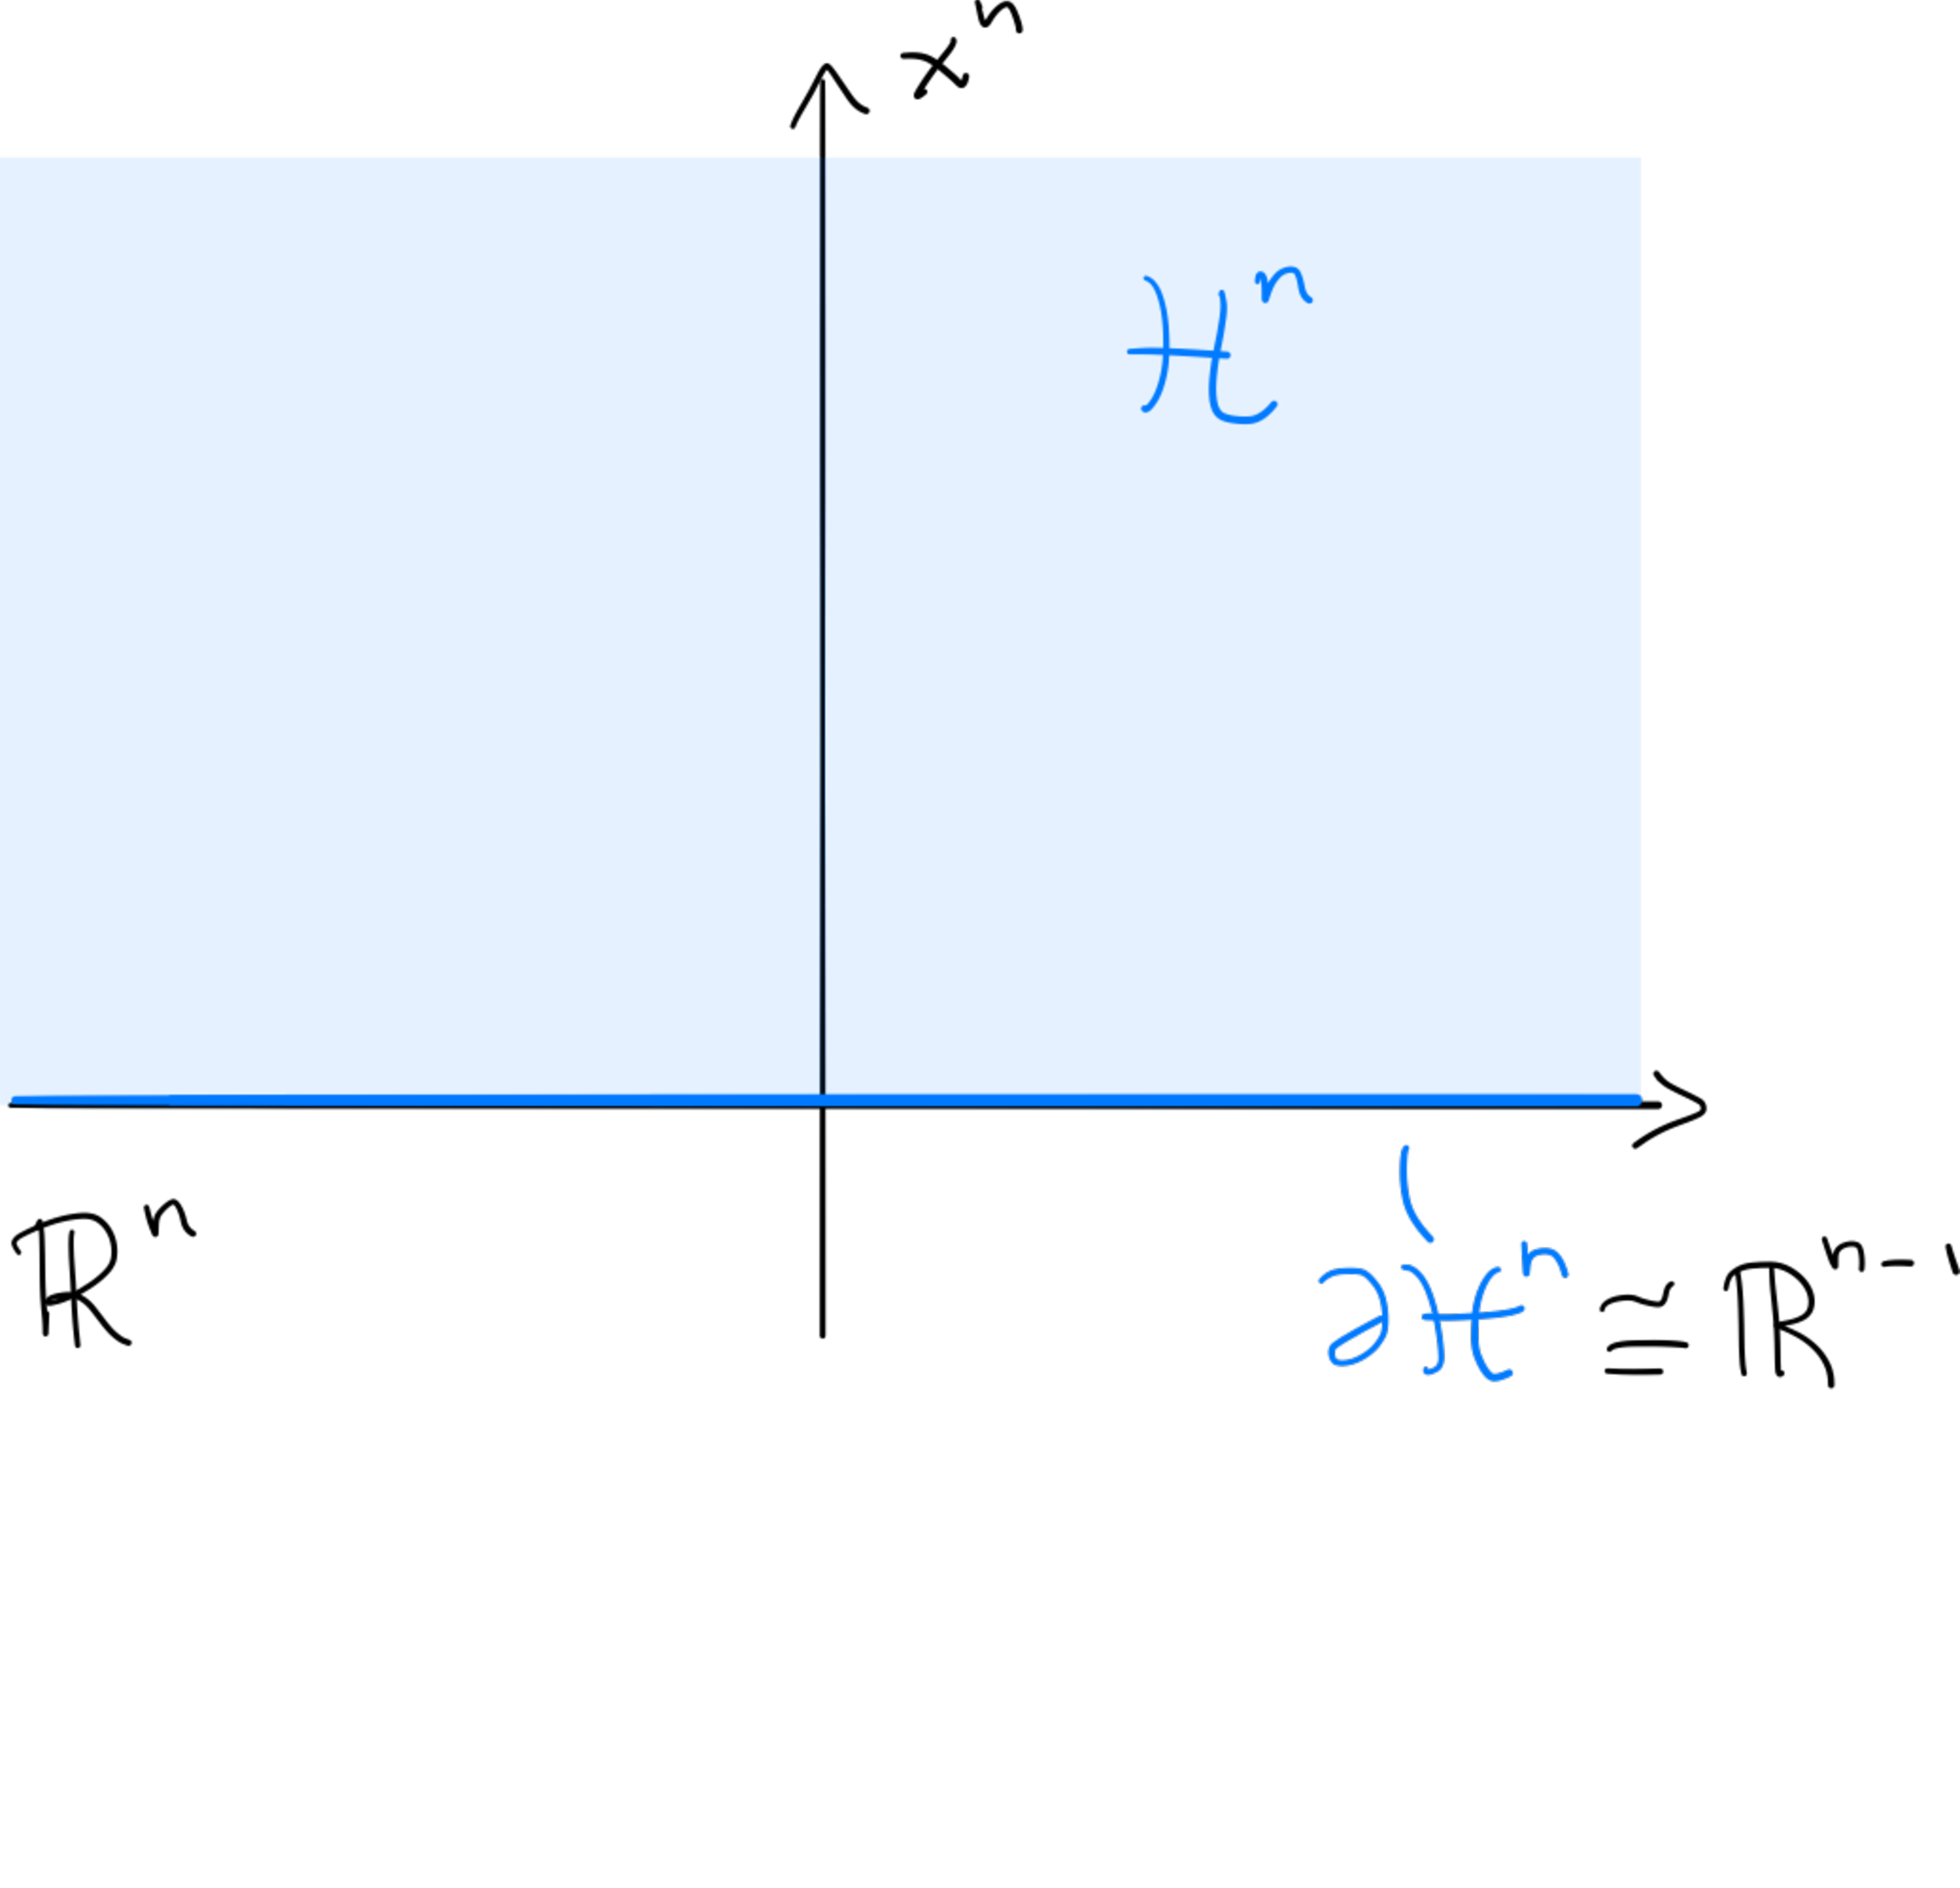
\includegraphics{1_4-upper_space.pdf}
\end{marginfigure}
\begin{equation}
  \cH^n = \R_+^n = \{x=(x^1, \ldots, x^n)\in\R^n\mid x^n \geq 0\},
\end{equation}
with its $(n-1)$-dimensional boundary
\begin{equation}
  \partial\cH^n = \{x=(x^1, \ldots, x^n)\in\R^n\mid x^n = 0\}
\end{equation}
and the topology inherited by $\R^n$, as a replacement for our local model $\R^n$.

\begin{definition}
  A topological space $M$ is a \emph{topological manifold with boundary} of dimension $n$, or topological $n$-manifold with boundary, if it has the following properties
  \begin{enumerate}[(i)]
    \item $M$ is a Hausdorff space;
    \item $M$ is second countable;
    \item $M$ is \emph{locally} homeomorphic to $\cH^n$, any point $x\in M$ has a neighbourhood that is homeomorphic to a (relatively) open\footnote{Recall that $U\subset\R^n_+$ is relatively open, that is open with respect to the relative topology, if there exist an open set $\tilde U\subset\R^n$ such that $U = \tilde U \cap \R^n_+$.} subset of $\R^n_+$.
  \end{enumerate}

  A \emph{chart} on $M$ is a pair $(U, \phi)$ consisting of an open set $U\subset M$ and a homeomorphism $\phi: U \to \phi(U)\subset \cH^n$.
\end{definition}

\begin{figure}
  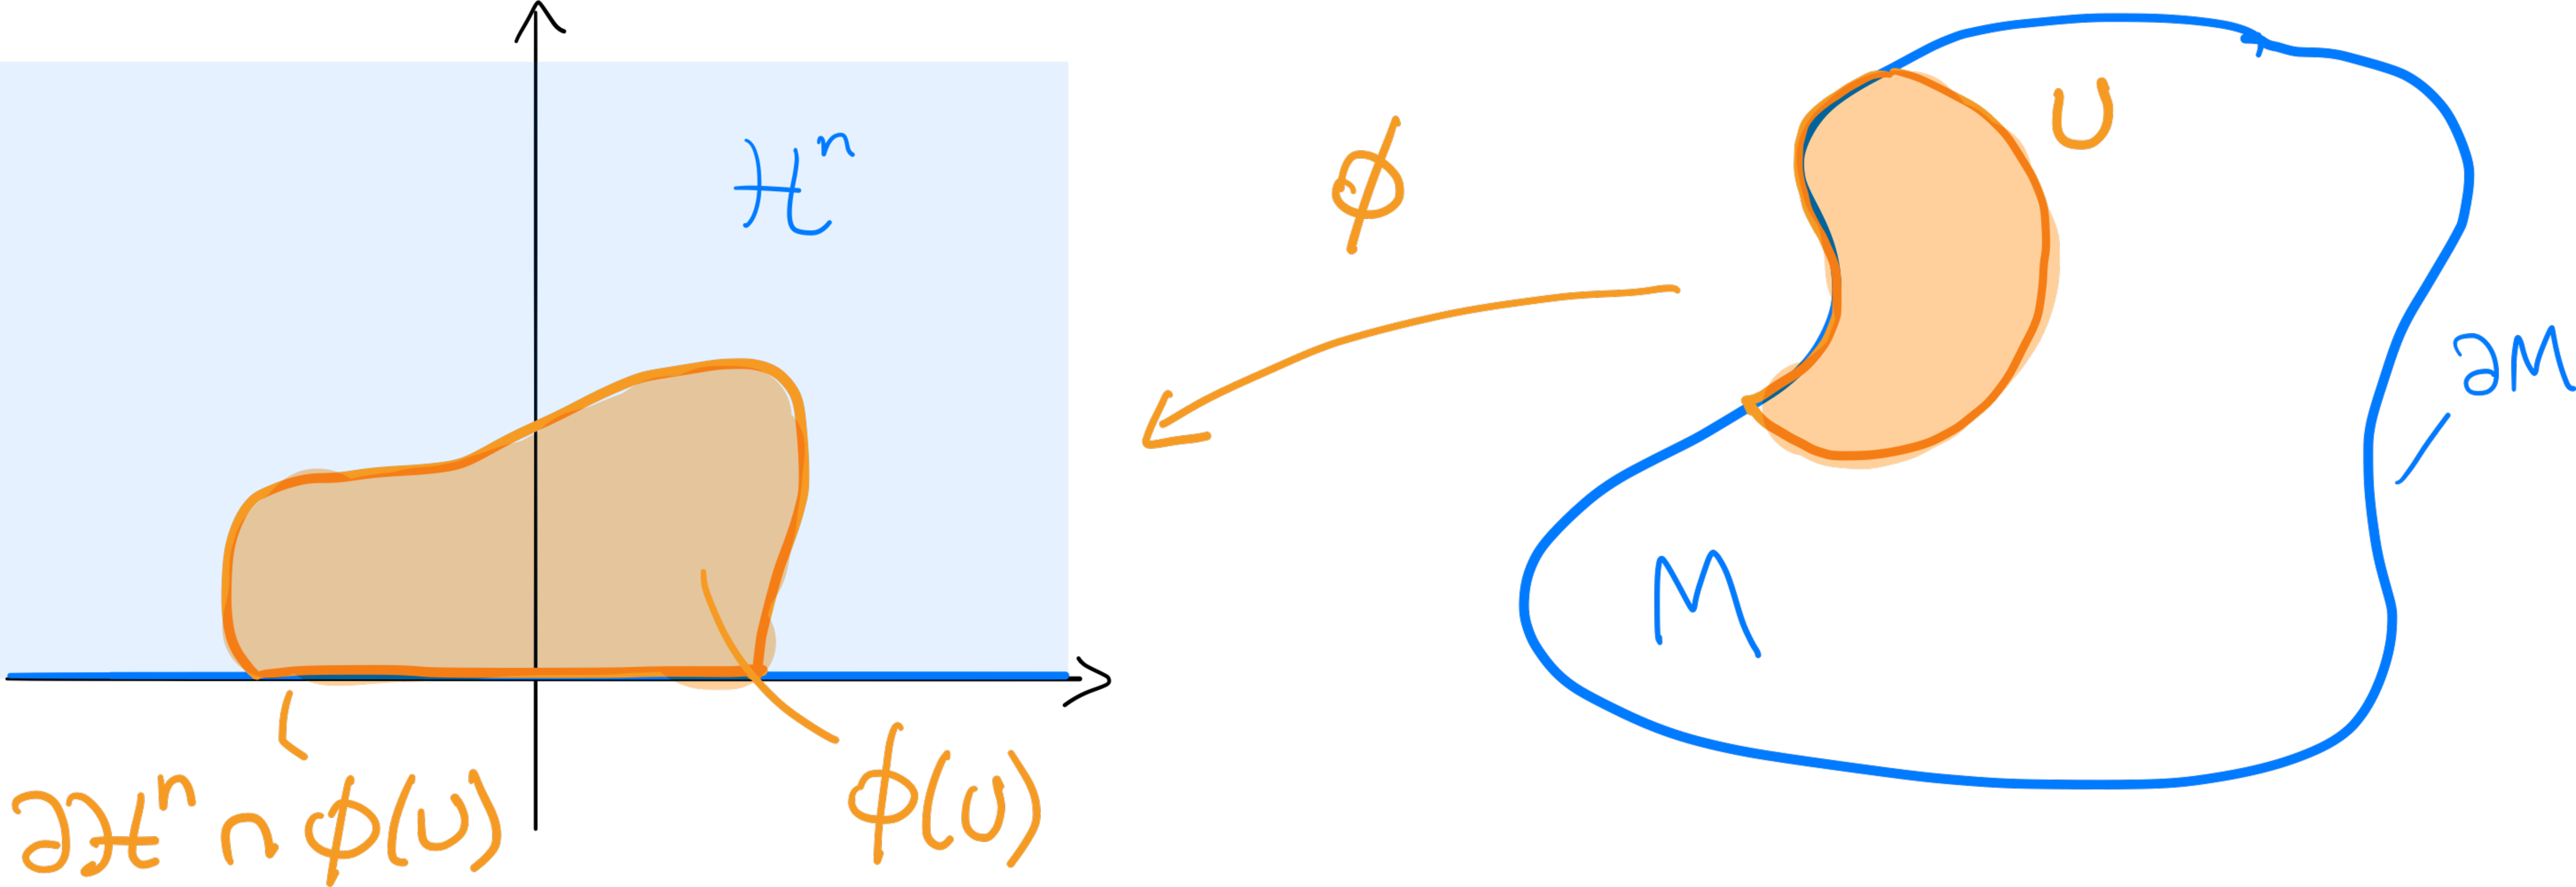
\includegraphics{1_4-mfld-w-bdry.pdf}
\end{figure}

We saw in Proposition~\ref{prop:uniqdiffeoinclusion} that differentiability is a local property, which means that is a property defined on open sets.
To clarify what it means to have differentiable structures on manifolds with boundary, we will thus need to clarify what it means for a function defined on $\cH^n$ to be differentiable at points on $\partial\cH^n$.
As it turns out, this is a minor modification of our previous definition that stems directly from the definition of the induced topology.

\begin{definition}
  Let $U\subset\cH^n$ be a relatively open set. A map $f: U\to\R^m$ is \emph{$r$-times continuously differentiable}, or of class $C^r$, if there exists an open set $\tilde U\in\R^n$ and a map $\tilde f\in C^r(\tilde U, \R^m)$ such that $U\subset\tilde U$ and $\tilde f|_U = f$.
  The function $f$ is said to be \emph{smooth}, or of class $C^\infty$, if $f$ is $r$-times continuously differentiable for all $r\geq 1$.
\end{definition}

With such definition at hand, one can define compatibility, smooth atlases and differentiable structures as in Definition~\ref{def:crcomp}, Definition~\ref{def:cratlas} and Definition~\ref{def:diffstr} by considering charts taking value in $\cH^n$.

\begin{definition}\label{def:diffmanifoldwb}
  A \emph{smooth manifold with boundary} of dimension $n$ is a pair $(M, \cA)$ of a topological $n$-manifold with boundary $M$ and a smooth differentiable structure $\cA = \{(U_\alpha, \phi_\alpha) \mid \alpha\in A\}$ on $M$.
  
  \marginnote[-2em]{The boundary $\partial M$ as defined by \eqref{def:bdry} can differ from its topological boundary as a subset of another topological space. For example the boundary $\partial\bS^1$ of the circle as a manifold is empty, but the boundary of the circle $\bS^1$ as a subset of $\R^2$ is $\bS^1$ itself.}
  The \emph{boundary} of $M$ is defined as
  \begin{equation}\label{def:bdry}
    \partial M := \bigcup_{\alpha\in A} \phi_\alpha^{-1}\left(\phi_\alpha(V_\alpha)\cap \partial\cH^n\right).
  \end{equation}
\end{definition}

\begin{proposition}\label{prop:bdwelldef}
  The boundary $\partial M$ is well defined\footnote{The same definition holds for topological manifolds, but showing that it is well defined is much more complicated and will be omitted.}.
\end{proposition}
\begin{proof}
  The statement follows if we show that the transition maps send boundary pieces to boundary pieces.
  It turns out that this fact is more general: for any diffeomorphism $f:U \to V$, where $U,V \subset\cH^n$ are relatively open, it holds that $x\in U\cap\partial\cH^n$ if and only if $f(x)\in V\cap\partial\cH^n$.

  Indeed, let $x\in U\cap(\cH^n\setminus\partial\cH^n)$ be a point in the interior of $U$. Expanding $f$ in Taylor series up to the first order, we have
  \begin{equation}
    f(x+h) = f(x) + Df|_x h + O(\|h\|).
  \end{equation}
  Since the differential $D f$ at $x$ is an isomorphism, there exist an open neighbourhood $\cO$ of $x$ such that $f(\cO)$ is open in $\R^n$ and thus $f(x)\in V\cap(\cH^n\cap\partial\cH^n)$.
\end{proof}

\begin{example}
  Let's go back to the closed interval $M=[a,b]\subset\R$. 
  With the atlas
  \begin{equation}
    \cA=\big\{
      \big([a,b), \; x\mapsto x-a\big),
      \big((a,b], \; x\mapsto b-x\big)
    \big\}
  \end{equation}
  it is a differentiable $1$-manifold with boundary $\partial M = \{a\} \cup \{b\} = \{a, b\}$.
\end{example}

Let's go back to our observation at the beginning of this section.
We started by observing that some objects seemed to be the ``sum'' of a boundary manifold and an interior manifold.
Can we make sense of such observation using our newly introduced definition?

\begin{proposition}
  Let $M$ be a differentiable $n$-manifold with boundary.
  Then $M\setminus\partial M$ and $\partial M$ inherit the structure of manifolds (without boundary) of dimensions $\dim(M\setminus\partial M)=n$ and $\dim(\partial M) = n-1$.
\end{proposition}
\begin{proof}
  Let $\cA = \{(U_\alpha,\phi_\alpha) \mid \alpha\in A\}$ be an atlas for $M$. 
  Then
  \begin{equation}
    \cA_\circ := \left\{
      \left(
        U_\alpha \cap (M\setminus\partial M),
        \phi_\alpha|_{U_\alpha \cap (M\setminus\partial M)}
        \right) \mid \alpha\in A
      \right\}
  \end{equation}
  is an atlas for $M\setminus\partial M$ where none of the charts contain points in $\partial\cH^n$.

  In a similar vein, an atlas for $\partial M$ is given by
  \begin{equation}
    \cA_\partial := \left\{
      \left(
        U_\alpha \cap \partial M,
        \phi_\alpha|_{U_\alpha \cap \partial M}
        \right) \mid \alpha\in A
      \right\},
  \end{equation}
  where
  \begin{equation}
    \phi_\alpha|_{U_\alpha \cap \partial M} : (U_\alpha \cap \partial M) \to \partial\cH^n\simeq\R^{n-1}
  \end{equation}
  by the proof of Proposition~\ref{prop:bdwelldef}.
\end{proof}

\begin{tcolorbox}
  Differentiable manifolds without boundary (cfr. Definition~\ref{def:diffmanifold}) can be thought as a special case of differentiable manifolds with boundary (cfr. Definition~\ref{def:diffmanifoldwb}) where the boundary happens to be empty.
  Therefore, with the exception of the beginning of Chapter~\ref{ch:2}, we will no-longer distinguish the two concepts: from now on, a manifold may have or may not have a boundary.
\end{tcolorbox}